%-------------------------------------------------------
% SLEPc Users Manual
%-------------------------------------------------------

\documentclass[titlepage,10pt,a4paper]{slepc}

%\usepackage[first,light,outline]{draftcopy}
\usepackage{graphicx}
\usepackage[square]{natbib}
\usepackage{fancyhdr}
\usepackage{fancyvrb}
\usepackage{subfigure}
\usepackage{caption}
\usepackage{xspace}
\usepackage{ae,aecompl}
\usepackage[active]{srcltx}
%\usepackage{hyperref}

\makeindex

%\includeonly{slepc1}

\newcommand{\slepcversion}{2.1.5}

% Paquets software
\newcommand{\pack}[1]{{\sc #1}\index{{\sc #1}}\xspace}
\newcommand{\packnoi}[1]{{\sc #1}\xspace}
\newcommand{\mpi}{\pack{mpi}}
\newcommand{\matlab}{{\sc matlab}\index{{\sc matlab}}\raisebox{1ex}{\tiny\textregistered}}
\newcommand{\blas}{\pack{blas}}
\newcommand{\blacs}{\pack{blacs}}
\newcommand{\arpack}{\pack{arpack}}
\newcommand{\parpack}{\pack{parpack}}
\newcommand{\lapack}{\pack{lapack}}
\newcommand{\itpack}{\pack{itpack}}
\newcommand{\sparskit}{\pack{sparskit}}
\newcommand{\petsc}{\pack{pets\rm c}}
\newcommand{\slepc}{\packnoi{slep\rm c}}
\newcommand{\trlan}{\pack{trlan}}
\newcommand{\lanso}{\pack{lanso}}
\newcommand{\planso}{\pack{planso}}
\newcommand{\blzpack}{\pack{blzpack}}
\newcommand{\aztec}{\pack{aztec}}
\newcommand{\pim}{\pack{pim}}
\newcommand{\isis}{\pack{isis{\small++}}}
\newcommand{\lopsi}{\pack{lopsi}}
\newcommand{\srrit}{\pack{srrit}}
\newcommand{\arncheb}{\pack{arncheb}}
\newcommand{\eispack}{\pack{eispack}}
\newcommand{\linpack}{\pack{linpack}}
\newcommand{\scalapack}{\pack{scalapack}}
\newcommand{\qmrpack}{\pack{qmrpack}}
\newcommand{\jdqz}{\pack{jdqz}}
\newcommand{\mpich}{\pack{mpich}}

% Misc
\newcommand{\slepchome}{http://www.grycap.upv.es/slepc}
\newcommand{\rutina}[1]{\texttt{#1}\index{\texttt{#1}}}
\newcommand{\ident}[1]{\texttt{#1}\index{\texttt{#1}}}
\newcommand{\findex}[1]{\index{\texttt{#1}}}
\newcommand{\flops}{flops}
\newcommand{\spup}{\emph{speed--up\/}}
\newcommand{\url}[1]{\texttt{#1}}
\newcommand{\K}{\mathcal{K}}
\newcommand{\LL}{\mathcal{L}}
\def\bbbr{{\rm I\!R}} 
\def\bbbc{{\mathchoice {\setbox0=\hbox{$\displaystyle\rm C$}\hbox{\hbox
to0pt{\kern0.4\wd0\vrule height0.9\ht0\hss}\box0}}
{\setbox0=\hbox{$\textstyle\rm C$}\hbox{\hbox
to0pt{\kern0.4\wd0\vrule height0.9\ht0\hss}\box0}}
{\setbox0=\hbox{$\scriptstyle\rm C$}\hbox{\hbox
to0pt{\kern0.4\wd0\vrule height0.9\ht0\hss}\box0}}
{\setbox0=\hbox{$\scriptscriptstyle\rm C$}\hbox{\hbox
to0pt{\kern0.4\wd0\vrule height0.9\ht0\hss}\box0}}}}
\newcommand{\Co}{\bbbc}
\newcommand{\Real}{\bbbr}

\setlength{\tabcolsep}{2mm}
\renewcommand{\arraystretch}{1.05} 
\setcounter{tocdepth}{3}
\renewcommand{\captionlabelfont}{\sl\sffamily}
\newcommand{\bibfont}{\small}

\newtheorem{algorithm}{Algorithm}[chapter]
\newcommand{\nosection}[1]{\chapter*{\sffamily\LARGE #1}\markboth{\scriptsize \sffamily #1}{}\addcontentsline{toc}{chapter}{#1}}

%VerbatimEnvironment%
\fvset{numbers=left,numbersep=6pt,stepnumber=5}
\newcommand{\MyVerbatimInput}[1]{\fvset{fontsize=\scriptsize}%
  \VerbatimInput{#1}%
  \fvset{fontsize=\normalsize}%
}

\begin{document}

\title{
 	\vspace*{-1cm}
	\framebox[12cm][l]{
	
\includegraphics[height=1.4cm]{upv.ps}
	\hfill
	\parbox[b]{4cm}{\begin{flushright}\vspace*{-7mm}\normalsize\sl\sffamily 
	Departamento de\\[-0.8mm] Sistemas Inform\'aticos\\[-0.8mm] 
	y Computaci\'on\\[0.8mm]
	\vspace{-2.5mm}\end{flushright}}
	\raisebox{3mm}{
\includegraphics[height=9mm,width=1.4cm]{dsic.ps}}
	}
	\\[2cm]
	\normalsize Technical Report DSIC-II/24/02
%	\\\normalsize Also available as ANL-XX/XX 
	\\[2cm]
	%\hrule
	\vspace*{6mm}
	{\Large\bf\sffamily 
	SLEPc Users Manual\\[2mm]}
	{\large\bf\sffamily 
	Scalable Library for Eigenvalue Problem Computations}\\[2mm]
	\vspace*{6mm}
	%\hrule
	\vspace*{6mm}
	\url{\slepchome}
	\\[6mm]
}

\author{
	Vicente Hern\'andez
	\\
	Jos\'e E. Rom\'an
	\\
	Vicent Vidal
	\\[2cm]
}

\date{
	To be used with \slepc \slepcversion\\
	May, 2003
}

{
\pagestyle{empty}
\maketitle
}

\setlength{\textheight}{14.99cm}
\setlength{\footskip}{2cm}
\setlength{\voffset}{2.3cm}

\pagestyle{empty}
\cleardoublepage

{
  \pagestyle{plain}
  \pagenumbering{roman}
%---------------------------------------------------
\subsection*{Abstract}

	This document describes \slepc, the {\em Scalable Library for Eigenvalue Problem Computations}, a software package for the solution of large sparse eigenproblems on parallel computers. It can be used for the solution of problems formulated in either standard or generalized form, as well as other related problems such as the singular value decomposition. 

	The emphasis of the software is on methods and techniques appropriate for problems in which the associated matrices are sparse, for example, those arising after the discretization of partial differential equations. Therefore, most of the methods offered by the library are projection methods or other methods with similar properties. Examples of these methods are Arnoldi, Lanczos and Subspace Iteration, to name a few. \slepc implements these basic methods as well as more sophisticated algorithms. It also provides built-in support for spectral transformations such as shift-and-invert.

	\slepc is a general library in the sense that it covers standard and generalized eigenvalue problems, both Hermitian and non-Hermitian, with either real or complex arithmetic.
	
	\slepc is built on top of \packnoi{pets\rm c}, the Portable, Extensible Toolkit for Scientific Computation \citep{Balay:2002:PUM}. It can be considered an extension of \packnoi{pets\rm c} providing all the functionality necessary for the solution of eigenvalue problems. This means that \packnoi{pets\rm c} must be previously installed in order to use \slepc. \packnoi{pets\rm c} users will find \slepc very easy to use, since it enforces the same programming paradigm. Those readers which are not acquainted with \packnoi{pets\rm c} are highly recommended to familiarize with it before proceeding with \slepc.

	This manual provides a general description of the package. In addition, manual pages for individual routines are included in the distribution in hypertext format.

	\slepc interfaces to some external software packages such as:
\begin{itemize}
\setlength{\itemsep}{-1pt}
\item \packnoi{arpack}, \url{http://www.caam.rice.edu/software/ARPACK}.
\item \packnoi{blzpack}, \url{http://www.nersc.gov/\~{}osni/\#Software}.
\item \packnoi{planso}, \url{http://www.nersc.gov/research/SIMON/planso.html}.
\item \packnoi{trlan}, \url{http://www.nersc.gov/\~{}kewu/trlan.html}.
\end{itemize}
These are all optional packages and do not need to be installed to use \slepc. See section \ref{sec:wrap} for details.

\subsubsection*{How to get \slepc}

	All the information related to \slepc can be found at the following web site:
	\begin{quote}
	\begin{center}
	\url{\slepchome}.
	\end{center}
	\end{quote}
	The distribution file is available for download at this site. Other information is provided there, such as installation instructions and contact information. Instructions for installing the software can also be found in section \ref{sec:inst} of this document.

	\packnoi{pets\rm c} can be downloaded from \url{http://www.mcs.anl.gov/petsc}.  \packnoi{pets\rm c} is supported, and information on contacting support can be found at this site.

\subsubsection*{Acknowledgements}

	We thank all the \packnoi{pets\rm c} team for their help. We also thank Barry Smith, David Keyes, Osni Marques, Tony Drummond and Rich Lehoucq for supporting this project.

	The development of the library has been partially funded by the Science and Technology Office of the Valencian Regional Government under grant number CTIDB/2002/54.

%---------------------------------------------------
  \setlength{\parskip}{0cm}
  \tableofcontents
}
\cleardoublepage
\pagenumbering{arabic}
\pagestyle{fancy}
\renewcommand{\chaptermark}[1]{\markboth{\scriptsize \sffamily {\bfseries\chaptername\ \thechapter.} #1}{}}
\renewcommand{\sectionmark}[1]{\markright{\scriptsize \sffamily {\bfseries\thesection.} #1}{}}
\fancyhead{}
\fancyhead[LE,RO]{\nouppercase{\rightmark}}
\fancyhead[LO,RE]{\nouppercase{\leftmark}}
\fancyfoot[C]{\scriptsize --- \thepage\ ---}
\renewcommand{\headrulewidth}{0.2pt}
\renewcommand{\footrulewidth}{0.2pt}

%-------------------------------------------------------
% SLEPc Users Manual
%-------------------------------------------------------
\chapter{\label{cap:int}Introduction}
%-------------------------------------------------------

\noindent \slepc, the {\em Scalable Library for Eigenvalue Problem Computations}, is a software package for the solution of large sparse eigenvalue problems on parallel computers. 

	Together with linear systems of equations, eigenvalue problems are a very important class of linear algebra problems. The need for the numerical solution of these problems arises in many situations in science and engineering. There is a strong demand for solving  problems associated with stability and vibrational analysis in practical applications, which are usually formulated as large sparse eigenproblems.

	Computing eigenvalues is essentially more difficult than solving linear systems of equations. This has resulted in a very active research activity in the area of computational methods for eigenvalue problems in the last years, with many remarkable achievements. 
	However, these state-of-the-art methods and algorithms are not easily transferred to the scientific community, and, apart from a few exceptions, scientists keep on using traditional well-established techniques.
	
	The reasons for this situation are manifold. First, new methods are increasingly complex and difficult to implement and therefore robust implementations must be provided by computational specialists, for example as software libraries. The development of such libraries requires to invest a lot of effort but sometimes they do not reach normal users due to a lack of awareness.
	
	In the case of eigenproblems, using libraries is not straightforward. It is usually recommended that the user understands how the underlying algorithm works and typically the problem is successfully solved only after several cycles of testing and parameter tuning. Methods are often specific for a certain class of eigenproblems (e.g. complex symmetric) and this leads to an explosion of available algorithms from which the user has to choose. Not all these algorithms are available in the form of software libraries, even less frequently with parallel capabilities.
	
	A further obstacle appears when these methods have to be applied in a large software project developed by inter-disciplinary teams. In this scenery, libraries must be able to interoperate with already existing software and with other libraries, possibly written in a different programming language. In order to cope with the complexity associated with such large software projects, libraries must be designed carefully in order to overcome hurdles such as different storage formats. In the case of parallel software, care must be taken also to achieve portability to a wide range of platforms with good performance and still retain flexibility and usability. 

	The \slepc library is an attempt to address this complexity and provides a set of tools that can be used to obtain a solution in many applications. \slepc is based on \petsc, the Portable, Extensible Toolkit for Scientific Computation \citep{Balay:2002:PUM}, and, therefore, a large percentage of the complexity is avoided since \slepc relies on \petsc\ for all low level implementation details. \slepc focuses on high level features structured around a few types of objects. It offers a growing number of solution methods as well as interfaces to integrate well-established eigenvalue packages such as \arpack.

%---------------------------------------------------
\section{Getting Started}

	\slepc is a general library for the solution of eigenvalue problems, in the sense that it covers standard and generalized eigenvalue problems, both Hermitian and non-Hermitian, with either real or complex arithmetic. This manual assumes that the reader is familiar with eigenvalue problems, their basic mathematical properties and the basic techniques and methods to solve them. A brief introduction to the topic is included in section \ref{sec:eig}. A nice introduction of eigenvalue problems and an overview of methods can be found in \citep{Golub:2000:EC2}.
	
	The emphasis of \slepc is on methods and techniques appropriate for problems in which the associated matrices are sparse, for example, those arising after the discretisation of partial differential equations. Therefore, most of the methods offered by the library are projection methods or other methods with similar properties. Examples of these methods are Arnoldi, Lanczos and Subspace Iteration, to name a few. A comprehensive description of state-of-the-art methods of this kind can be found in \citep{Bai:2000:TSA}. \slepc contains implementations of the basic methods as well as a growing number of more sophisticated algorithms.

	The Portable, Extensible Toolkit for Scientific Computation (\petsc) uses modern programming paradigms to ease the development of large-scale scientific application codes in Fortran, C, and C++ and provides a powerful set of tools for the numerical solution of partial differential equations and related problems on high-performance computers. \slepc is based on \petsc, and this means that \petsc\ must be previously installed in order to use \slepc. \petsc\ users will find \slepc very easy to use, since it enforces the same programming paradigm. Those readers which are not acquainted with \petsc\ are highly recommended to familiarize with it before proceeding with \slepc. An introduction to \petsc\ is included in section \ref{sec:petsc}.

	\slepc can be considered an extension of \petsc\ providing all the functionality necessary for the solution of eigenvalue problems. Figure \ref{fig:slepc} shows a diagram of all the different objects included in \petsc\ (on the left) and those added by \slepc (on the right). \petsc\ is a prerequisite for \slepc and users should be familiar with basic concepts such as vectors and matrices in order to use \slepc. Therefore, together with this manual we recommend to use the \petsc\ Users Manual \citep{Balay:2002:PUM}.

\begin{figure}[t]
\centering
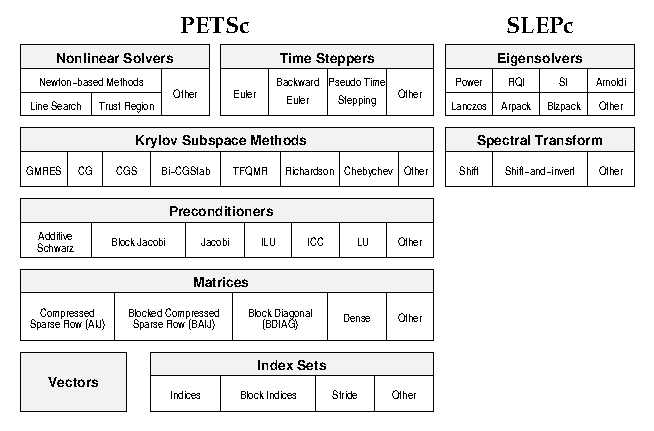
\includegraphics[width=12cm]{slepc-fig.eps}
\caption{\label{fig:slepc}Numerical components of \petsc\ and \slepc.}
\end{figure}

The complete \slepc distribution, users manual, manual pages, and additional information are available via the \slepc home page at 
	\begin{quote}
	\begin{center}
	\url{\slepchome}.
	\end{center}
	\end{quote}
The \slepc home page also contains details regarding installation, new features and changes in recent versions of \slepc, and more information.

Within the \slepc distribution, the directory 
\Verb!${SLEPC_DIR}/docs!
%\texttt{\$\{SLEPC\_DIR\}/docs}
 contains all the documentation of the library. Manual pages for all \slepc functions can be accessed on-line at \url{\slepchome/document.htm}. These manual pages provide hyperlinked indices (organized by both concepts and routine names) to the source code and enable easy movement among related topics.  The file \texttt{slepc.ps} contains the Postscript form of the \slepc Users Manual (this document). A PDF version is also available.

\medskip
\textbf{Note to Fortran Programmers}: As in the case of \petsc, in this manual  all the examples and calling sequences are given for the C/C++ programming languages. However, Fortran programmers can use most of the functionality of \slepc and \petsc\ from Fortran, with only minor differences in the user interface. Section \ref{sec:fortran} provides a discussion of the differences between using \slepc from Fortran and C, as well as complete Fortran examples. 

%---------------------------------------------------
\section{Installation}
\label{sec:inst}

	This section gives an overview of the installation procedure. For full installation instructions see \url{\slepchome/install.htm}.

	Previously to the installation of \slepc, the system must have an appropriate version of \petsc\ installed. Table \ref{tab:ver} shows a list of \slepc versions and their corresponding \petsc\ versions. \slepc versions marked as major releases are those which incorporate some new functionality. The rest are just adaptations required for a new \petsc\ release and may also include bug fixes.

\begin{table}[ht]
\centering
\begin{tabular}{cccccc} \hline
\slepc version & \petsc\ version & Major & Status & Release date \\ \hline\hline
2.1.0 & 2.1.0 &   $ \star$   & Not released     & - \\ \hline
2.1.1 & 2.1.1 &   & Released & Dec 2002 \\ 
      & 2.1.2 &   &          &   \\ 
      & 2.1.3 &   &          &   \\ \hline
2.1.5 & 2.1.5 &   & Released & May 2003 \\ \hline
      & 2.1.6 &   &          &          \\ \hline
2.2.0 & 2.2.0 & $\star$ & Released & Apr 2004 \\ \hline
\end{tabular}
\caption{\label{tab:ver} Correspondence between \slepc and \petsc\ releases.}
\end{table}

	Although installing \petsc\ can be tricky some times, in general it is very easy. The user simply sets the environment variables \ident{PETSC\_DIR} and \ident{PETSC\_ARCH} and types \texttt{make}. Apart of this, some customization may be necessary, see the \petsc\ documentation for details.

	The installation process for \slepc is very similar. The main steps are described next. Note that prior to this steps, optional packages must have been installed. If any of these packages is installed afterwards, recompilation is necessary. Refer to \url{\slepchome/install.htm} or to section \ref{sec:wrap} for details about installation of some of these packages.

\begin{enumerate}
	\item Unbundle the distribution file \Verb!slepc.tgz! with a usual command such as \Verb!gunzip -c slepc.tgz | tar xvf -!. This will create a directory and unpack the software there.
	\item Refer to \url{\slepchome/download.htm} for available patches to the latest \slepc release.
	\item Set the environment variable \ident{SLEPC\_DIR} to the full path of the \slepc home directory, for example,
	\begin{Verbatim}[fontsize=\small]
	setenv SLEPC_DIR /home/username/slepc-2.2.0
	\end{Verbatim}
	In addition to this variable, \ident{PETSC\_DIR} and \ident{PETSC\_ARCH} must also be set correctly, the first one pointing to the \petsc\ home directory and the other containing the selected architecture (remember that \petsc\ allows several versions compiled for different architectures to coexist in the same directory tree).
	\item Edit the file \Verb!${SLEPC_DIR}/bmake/${PETSC_ARCH}/packages! to indicate the local installation of optional software packages such as \arpack. If there exists no directory named \Verb!bmake/${PETSC_ARCH}! for the value of \Verb!${PETSC_ARCH}! you are using, then create it similar to the existing ones.
	\item In the \slepc home directory, type
	\begin{Verbatim}[fontsize=\small]
	make BOPT=g
	\end{Verbatim}
      to build a debugging version of \slepc, or
	\begin{Verbatim}[fontsize=\small]
	make BOPT=O
	\end{Verbatim}
      to build an optimized version of the \slepc libraries. The flag \ident{BOPT} determines what type of libraries are built (i.e., specifies compiler options). Other available alternatives are \Verb!BOPT=[g_complex,O_complex]! for complex numbers versions (see section \ref{sec:complex}).
	\item If the installation went smoothly, then try running some test examples with the command
	\begin{Verbatim}[fontsize=\small]
	make BOPT=g slepc_testexamples >& examples_log 
	\end{Verbatim}
     Examine the file \Verb!examples_log! for any obvious errors or problems.
	\item The Fortran libraries are built automatically during the installation outlined above. To compile and test the Fortran examples, use the command
	\begin{Verbatim}[fontsize=\small]
	make BOPT=g slepc_testfortran >& fortran_log
	\end{Verbatim}
\end{enumerate}
	
	For details about availability of \slepc on Windows platforms, see the up-to-date information in \url{\slepchome/install.htm}.
%---------------------------------------------------
\section{Running \slepc Programs}

Before using \slepc, the user must first set the environment variable
\ident{SLEPC\_DIR}, indicating the full path of the \slepc home
directory. For example, under the UNIX C shell a command of the form
	\begin{Verbatim}[fontsize=\small]
	setenv SLEPC_DIR /software/slepc
	\end{Verbatim}
can be placed in the user's \Verb!.cshrc! file. 
In addition, the user must set the two environment
variables required by \petsc, that is, \ident{PETSC\_DIR}, to indicate the full path of the \petsc\ installation, and \ident{PETSC\_ARCH} to specify the architecture (e.g., \texttt{rs6000},
\texttt{solaris}, \texttt{IRIX}, etc.)  on which \petsc\ is being used.  The utility
 \Verb!${PETSC_DIR}/bin/petscarch! can be used for this purpose.  For example,
	\begin{Verbatim}[fontsize=\small]
	setenv PETSC_ARCH `$PETSC_DIR/bin/petscarch`
	\end{Verbatim}
can be placed in a \Verb!.cshrc! file.  Thus, even if several machines of different
types share the same filesystem, \ident{PETSC\_ARCH} will be set correctly
when logging into any of them. 

All \petsc\ programs use the MPI (Message Passing Interface) standard
for message-passing communication \citep{MPI-Forum:1994:MMI}.  Thus, to execute
\slepc programs, users must know the procedure for launching MPI jobs
on their selected computer system(s).  For instance, when using the
\mpich\ implementation of MPI and many others, the \texttt{mpirun} command can be used to initiate a program as in the following example that uses eight processors:
	\begin{Verbatim}[fontsize=\small]
	mpirun -np 8 slepc_program [arguments]
	\end{Verbatim}

All \petsc-compliant programs support the use of the \Verb!-h!
or \Verb!-help! option as well as the \Verb!-v! or \Verb!-version! option. In the case of \slepc programs, specific information for \slepc is also displayed.

%---------------------------------------------------
\section{Writing \slepc Programs}

Most \slepc programs begin with a call to \rutina{SlepcInitialize}
	\begin{Verbatim}[fontsize=\small]
	SlepcInitialize(int *argc,char ***argv,char *file,char *help);
	\end{Verbatim}
which initializes \slepc, \petsc\ and MPI. This subroutine is very similar to \rutina{PetscInitialize}, and the arguments have the same meaning. In fact, internally \rutina{SlepcInitialize} calls \rutina{PetscInitialize}.
In Fortran the initialization command has the form
	\begin{Verbatim}[fontsize=\small]
	SlepcInitialize(character file,integer ierr)
	\end{Verbatim}

After this initialization, \slepc programs can use communicators defined by \petsc. In most cases users can employ the communicator \ident{PETSC\_COMM\_WORLD} to indicate all processes in a given run and \ident{PETSC\_COMM\_SELF} to indicate a single process. MPI provides routines for generating new communicators consisting of subsets of processors, though most users rarely need to use these. \slepc users need not program much message passing directly
with MPI, but they must be familiar with the basic concepts of message
passing and distributed memory computing.

All \slepc routines return an integer indicating whether an error has
occurred during the call.  The error code is set to be nonzero if an
error has been detected; otherwise, it is zero.  For the C/C++
interface, the error variable is the routine's return value, while for
the Fortran version, each \petsc\ routine has as its final argument an
integer error variable. 

All \slepc programs should call \rutina{SlepcFinalize}
as their final (or nearly final) statement, as given below in the C/C++
and Fortran formats, respectively:
	\begin{Verbatim}[fontsize=\small]
	ierr = SlepcFinalize();
	call SlepcFinalize(ierr)
	\end{Verbatim}
This routine handles options to be called at the conclusion of
the program, and calls \rutina{PetscFinalize}
if \rutina{SlepcInitialize}
began \petsc.


%---------------------------------------------------
\section{Simple \slepc Example}
\label{sec:simpleex}

To help the user start using \slepc immediately, a simple example is listed next which solves an eigenvalue problem associated with the
one-dimensional Laplacian operator discretized with finite differences.  This
example can be found in \Verb!${SLEPC_DIR}/src/examples/ex1.c!.
Following the code we highlight a few of the most important parts of this example.  

\MyVerbatimInput{${SLEPC_DIR}/src/examples/ex1.c}

\subsubsection*{Include Files}

The C/C++ include files for \slepc should be used via statements such as
	\begin{Verbatim}[fontsize=\small]
	#include "slepceps.h"
	\end{Verbatim}
where \Verb!slepceps.h! is the include file for the \ident{EPS} component.
Each \slepc program must specify an
include file that corresponds to the highest level \slepc objects
needed within the program; all of the required lower level include
files are automatically included within the higher level files. 
For
example, \Verb!slepceps.h! includes \Verb!slepcst.h! (spectral transformations),
and \Verb!slepc.h! (base \slepc file).  
The \slepc include files are located in the directory 
\Verb!${SLEPC_DIR}/include!.

\subsubsection*{The Options Database}

All the \petsc\ functionality related to the options database is available in \slepc. This allows the user to input control data
at run time very easily. In this example the command
\Verb!PetscOptionsGetInt(PETSC_NULL,"-n",&n,PETSC_NULL);! checks whether the user has
provided a command line option to set the value of \Verb!n!, the
problem dimension.  If so, the variable \Verb!n! is set accordingly;
otherwise, \Verb!n! remains unchanged.

\subsubsection*{Vectors and Matrices}

Usage of matrices and vectors in \slepc is exactly the same as in \petsc.
The user can create a new parallel or sequential matrix, \texttt{A}, which
has \texttt{M} global rows and \texttt{N} global columns, with the routine
\rutina{MatCreate}
	\begin{Verbatim}[fontsize=\small]
	MatCreate(MPI_Comm comm,int m,int n,int M,int N,Mat *A);
	\end{Verbatim}
where the matrix format can be specified at runtime. The example creates a matrix, sets the nonzero values with \rutina{MatSetValues} and then assembles it.

\subsubsection*{Eigensolvers}

Usage of eigensolvers is very similar to other kinds of solvers provided by \petsc.
After creating the matrix (or matrices) that define the problem,
$Ax = kx$ (or $Ax=kBx$), the user can then use \ident{EPS} to solve the system 
with the following sequence of commands: 
\findex{EPSCreate} \findex{EPSSetOperators}
\findex{EPSSetFromOptions} \findex{EPSSolve} \findex{EPSDestroy}
	\begin{Verbatim}[fontsize=\small,numbers=none]
	EPSCreate(MPI_Comm comm,EPS *eps);
	EPSSetOperators(EPS eps,Mat A,Mat B);
	EPSSetFromOptions(EPS eps);
	EPSSolve(EPS eps);
	EPSGetIterationNumber(EPS eps,int *its);
	EPSGetConverged(EPS eps, int *nconv);
	EPSGetEigenpair(EPS eps,int i,PetscScalar *kr,PetscScalar *ki,Vec xi,Vec xr);
	EPSDestroy(EPS eps);
	\end{Verbatim}
The user first creates the \ident{EPS} context and sets the operators
associated with the eigensystem. The user then sets various options for
customized solution, solves the problem, retrieves the solution, 
and finally destroys the \ident{EPS} context.
Chapter~\ref{cap:eps} describes in detail the \ident{EPS} package, including
the options database which enables the user to customize the solution
process at runtime by selecting the solution algorithm and also specifying the convergence tolerance, setting various monitoring routines, etc.

\subsubsection*{Spectral Transformation}

In the example program above there is no explicit reference to spectral transformations. However, an \ident{ST} object is handled internally so that the user is able to request different transformations such as shift-and-invert.
Chapter~\ref{cap:st} describes the \ident{ST} package in detail.

\subsubsection*{Error Checking}

All \slepc routines return an integer indicating whether an error
has occurred during the call.  The \petsc\ macro \Verb!CHKERRQ(ierr)!
checks the value of \Verb!ierr! and calls the \petsc\ error handler
upon error detection.  \Verb!CHKERRQ(ierr)! should be used in all
subroutines to enable a complete error traceback. See the \petsc\ manual 
for full details.

\subsubsection*{Writing Application Codes with \slepc}

The examples provided in the \Verb!src/examples! directory demonstrate the software usage
and can serve as templates for developing
custom applications.
To write a new application program using \slepc, we suggest the
following procedure:
\begin{enumerate}
\item Install and test \slepc according to the instructions at the \slepc web site.
\item Copy the \slepc example 
      that corresponds to the class of problem of interest (e.g.,
      singular value decomposition).
\item Copy the corresponding makefile within the example directory;
      compile and run the example program.
\item Use the example program as a starting point for developing a custom code.
\end{enumerate}


%---------------------------------------------------
\section{Directory Structure}

	The directory structure of the \slepc software is very similar to that in \petsc. The root directory of \slepc contains the following directories:
\begin{description}
\item[\texttt{bmake}] - Base \slepc makefile directory. Includes subdirectories for various architectures.
\item[\texttt{docs}] - All documentation for \slepc, including this manual. The subdirectory \texttt{manualpages} contains the on-line manual pages of each \slepc routine.
\item[\texttt{include}] - All include files for \slepc that are visible to the user.
\item[\texttt{include/finclude}] - \slepc include files for Fortran programmers using the .F suffix.
\item[\texttt{lib}] - Location of all the generated libraries for each combination of \texttt{BOPT} and architecture.
\item[\texttt{src}] - The source code for all \slepc components, which currently includes
\begin{description}
\item \texttt{sys} - general system-related routines.
\item \texttt{eps} - eigenvalue problem solver.
\item \texttt{st} - spectral transformation.
\item \texttt{fortran} - Fortran interface stubs.
\item \texttt{examples} - example programs.
\item \texttt{mat/examples} - matrices used by some examples.
\end{description}
\end{description}

Each \slepc source code component directory has the following subdirectories:
\begin{description}
\item \texttt{interface} - The calling sequences for the abstract interface to the components. Code here does not know about particular implementations.
\item \texttt{impls} - Source code for one or more implementations.
\end{description}


%-------------------------------------------------------
% SLEPc Users Manual
%-------------------------------------------------------
\chapter{\label{cap:eps}EPS: Eigenvalue Problem Solver}
%-------------------------------------------------------

\noindent The Eigenvalue Problem Solver (\ident{EPS}) is the main object provided by \slepc. It is used to specify an eigenvalue problem, either in standard or generalized form, and provides uniform and efficient access to all of the eigensolvers included in the package. Conceptually, the level of abstraction occupied by \ident{EPS} is similar to other solvers in \petsc\ such as \ident{KSP} for solving linear systems of equations.
	
\section{General Description}

	The \ident{EPS} module can be used to solve eigenvalue problems. In the standard formulation, the problem consists in the determination of $\lambda\in\Co$ for which the equation
\begin{equation}Ax=\lambda x\;\;\end{equation}
has nontrivial solution, where $A\in\Co^{n\times n}$ and $x \in \Co^n$. The scalar $\lambda$ and the vector $x$ are called eigenvalue and eigenvector, respectively. Note that they can be complex even when the matrix is real.
\slepc can also solve eigenvalue problems in generalized form,
\begin{equation}Ax=\lambda Bx\;\;,\end{equation}
where $B\in\Co^{n\times n}$.

	The methods provided by \slepc are appropriate for large sparse eigenproblems and typically only use matrix $A$ in matrix-vector products of the form $w=Av$, or $w=B^{-1}\!Av$ in the generalized case. In these two cases, the matrices $A$ and $B^{-1}\!A$, respectively, will be referred to as the {\em operator\/} matrix. Therefore, the implemented methods apply the operator to a set of vectors repeatedly until the approximations to the eigenpairs are sufficiently accurate. The operator can adopt yet other different forms if spectral transformations are used, as explained in chapter \ref{cap:st}.

	\slepc assumes that only a subset of the eigenvalues must be computed. The user specifies how many of them and also in which part of the spectrum they are to be sought.
	
%---------------------------------------------------
\section{Basic Usage}

	The \ident{EPS} module is used in a similar way as other \petsc\ modules such as \ident{KSP}. All the information related to an eigenvalue problem is handled via a context variable. The usual object management functions are available (\ident{EPSCreate}, \ident{EPSDestroy}, \ident{EPSView}, \ident{EPSSetFromOptions}). In addition, the \ident{EPS} object provides functions for setting several parameters such as the number of eigenvalues to compute, the dimension of the subspace, the requested tolerance and the maximum number of iterations allowed. The user can also specify other things such as the orthogonalization technique or the portion of the spectrum of interest.

	The solution of the problem is obtained in several steps. First of all, the matrices associated to the eigenproblem are specified via \ident{EPSSetOperators}. Then, a call to \ident{EPSSolve} is done which invokes the subroutine for the selected eigensolver. \ident{EPSGetConverged} can be used afterwards to determine how many of the requested eigenpairs have converged to working precision. \ident{EPSGetEigenpair} is finally used to retrieve the eigenvalues and eigenvectors. 

	In order to illustrate the basic functionality of the \ident{EPS} package, a simple example is shown in figure \ref{fig:ex-eps}. The example code implements the solution of a simple standard eigenvalue problem. Code for setting up the matrix $A$ is not shown and error-checking code is omitted.

\begin{figure}[t]
\begin{Verbatim}[fontsize=\small,numbers=left,numbersep=6pt,xleftmargin=15mm]
Vec         xr, xi;       /* basis vectors */
Mat         A;            /* operator matrix */
EPS         eps;          /* eigenproblem solver context */
PetscReal   error;
PetscScalar kr, ki;
int         its, nconv;

EPSCreate( PETSC_COMM_WORLD, &eps );
EPSSetOperators( eps, A, PETSC_NULL );
EPSSetFromOptions( eps );
EPSSolve( eps );
EPSGetIterationNumber( eps, &its );
EPSGetConverged( eps, &nconv );
EPSGetEigenpair( eps, j, &kr, &ki, xr, xi );
EPSComputeRelativeError( eps, i, &error );
EPSDestroy( eps );
\end{Verbatim}
\caption{\label{fig:ex-eps}Example code for basic solution with \ident{EPS}.}
\end{figure}

	All the operations of the program are done over a single \ident{EPS} object. This solver context is created in line 8 with the command 
	\findex{EPSCreate}
	\begin{Verbatim}[fontsize=\small]
	EPSCreate(MPI_Comm comm,EPS *eps);
	\end{Verbatim}
	Here \texttt{comm} is the MPI communicator, and \texttt{eps} is the newly formed solver context. Before actually solving an eigenvalue problem with \ident{EPS}, the user must specify the matrices associated to the problem, as in line 9, with the following routine
	\findex{EPSSetOperators}
	\begin{Verbatim}[fontsize=\small]
	EPSSetOperators(EPS eps,Mat A,Mat B);
	\end{Verbatim}
	The only necessary change to the example code in order to solve a generalized problem is to provide matrix $B$ as the third argument to the call. The matrices specified in this call can be in any \petsc\ format. In particular, \ident{EPS} allows the user to solve matrix-free problems by specifying matrices created via \ident{MatCreateShell}. A more detailed discussion of this issue is given in section \ref{sec:supported}.

	After setting the problem matrices, the value of the different options could be set by means of a function call such as \ident{EPSSetTolerances} (explained later in this chapter). After this, a call to \ident{EPSSetFromOptions} should be made as in line 10, 
	\findex{EPSSetFromOptions}
	\begin{Verbatim}[fontsize=\small]
	EPSSetFromOptions(EPS eps);
	\end{Verbatim}
	The effect of this call is that options specified at runtime in the command line are passed to the \ident{EPS} object appropriately. In this way, the user can easily experiment with different combinations of options without having to recompile. All the available options as well as the associated function calls are described later in this chapter.

	Line 11 launches the solution algorithm, simply with the command
	\findex{EPSSolve}
	\begin{Verbatim}[fontsize=\small]
	EPSSolve(EPS eps);
	\end{Verbatim}
	The subroutine which is actually invoked depends on which solver has been selected by the user. 
        
        All the data associated to the solution of the eigenproblem is kept internally. The function
	\findex{EPSGetIterationNumber}
	\begin{Verbatim}[fontsize=\small]
        EPSGetIterationNumber(EPS eps,int *its);
	\end{Verbatim}
        retrieves in the parameter \texttt{its} either the iteration number at which convergence was successfully reached, or the \emph{negative} of the iteration at which a problem was detected. And the function
	\findex{EPSGetConverged}
	\begin{Verbatim}[fontsize=\small]
	EPSGetConverged(EPS eps,int *nconv);
	\end{Verbatim}
	queries how many eigenpairs have converged to working precision. The solution of the eigenproblem is retrieved in line 14 with one or serveral calls to the following function
	\findex{EPSGetEigenpair}
	\begin{Verbatim}[fontsize=\small]
	EPSGetEigenpair(EPS eps,int j,PetscScalar *kr,PetscScalar *ki,
               Vec xr, Vec xi);
	\end{Verbatim}
	\label{GetEigenpair}
	This function returns the $j$-th solution of the eigenproblem. \texttt{kr} and \texttt{ki} receive the real and imaginary parts of the eigenvalue, while \texttt{xi} and \texttt{xr} receive the real and imaginary parts of the associated eigenvector. Therefore, the $j$-th eigenvalue is \texttt{kr}$+\,i\cdot$\texttt{ki} and the $j$-th eigenvector is stored in the \texttt{Vec} objects \texttt{xr} and \texttt{xi}. 
	[Note: see section \ref{sec:complex} for a detailed discussion of this issue.] 
	
	In line 15 of the example the relative residual error $\|Ax_j\!-\!\lambda_jBx_j\|/\|\lambda_jx_j\|$ associated to the $j$-th eigenpair is computed with a call to
	\findex{EPSComputeRelativeError}
	\begin{Verbatim}[fontsize=\small]
	EPSComputeRelativeError(EPS eps,int j,PetscReal *error);
	\end{Verbatim}

	Once the \ident{EPS} context is no longer needed, it should be destroyed with the command
	\findex{EPSDestroy}
	\begin{Verbatim}[fontsize=\small]
	EPSDestroy(EPS eps);
	\end{Verbatim}
%	Note that this will also release the storage allocated for the solution (eigenvalues and eigenvectors).

	The above procedure is sufficient for general use of the \ident{EPS} package. As in the case of the \ident{KSP} solver, the user can optionally explicitly call 
	\findex{EPSSetUp}
	\begin{Verbatim}[fontsize=\small]
	EPSSetUp(EPS eps);
	\end{Verbatim}
before calling \ident{EPSSolve} to perform any setup required for the eigensolver.

	Internally, the \ident{EPS} object works with an \ident{ST} object (spectral transformation, described in chapter \ref{cap:st}). To allow application programmers to set any of the spectral transformation options directly within the code, the following routine is provided to extract the \ident{ST} context,
	\findex{EPSGetST}
	\begin{Verbatim}[fontsize=\small]
	EPSGetST(EPS eps,ST *st);
	\end{Verbatim}
	
	With the command
	\findex{EPSView}
	\begin{Verbatim}[fontsize=\small]
	EPSView(EPS eps,PetscViewer viewer);
	\end{Verbatim}
it is possible to examine the information relevant to the \ident{EPS} object, such as the value of the different parameters, including also data related to the associated \ident{ST} object.

	The options database key \Verb!-eps_plot_eigs! instructs \slepc to plot the computed approximations of the eigenvalues in an X display after the solution process.

%---------------------------------------------------
\section{Defining the Problem}

	From the information provided by the user, \slepc tries to guess the kind of problem that is to be solved. For instance, if the user provides two matrices then the problem is generalized. However, the user has also the ability to specify explicitly the problem type. This could be used for instance to force a non-Hermitian version of an algorithm even when the matrix is Hermitian, or when the guess made by \slepc is not correct. However, normal usage will not require this.

The problem type can be specified at run time with the corresponding command line key (see table \ref{tab:ptype}) or within the program with the function
	\findex{EPSSetProblemType}
	\begin{Verbatim}[fontsize=\small]
	EPSSetProblemType(EPS eps,EPSProblemType type);
	\end{Verbatim}

\begin{table}[t]
\centering
{\small \begin{tabular}{lll}
Problem Type              & \ident{EPSProblemType} & Command line key\\\hline
Hermitian                 & \texttt{EPS\_HEP}         & \texttt{-eps\_hermitian}\\
Generalized Hermitian     & \texttt{EPS\_GHEP}        & \texttt{-eps\_gen\_hermitian}\\
Non-Hermitian             & \texttt{EPS\_NHEP}        & \texttt{-eps\_non\_hermitian}\\
Generalized Non-Hermitian & \texttt{EPS\_GNHEP}       & \texttt{-eps\_gen\_non\_hermitian}\\\hline
\end{tabular} }
\caption{\label{tab:ptype}Problem types considered in \ident{EPS}.}
\end{table}

	The type of the problem can be determined with the functions
	\findex{EPSIsGeneralized} \findex{EPSIsHermitian}
	\begin{Verbatim}[fontsize=\small]
	EPSIsGeneralized(EPS eps,PetscTruth *gen);
	EPSIsHermitian(EPS eps,PetscTruth *her);
	\end{Verbatim}

	The user can specify which eigenvalues to compute. The default is to compute only one eigenvalue (and eigenvector), in particular, the dominant one (largest in magnitude). The function
	\findex{EPSSetDimensions}
	\begin{Verbatim}[fontsize=\small]
	EPSSetDimensions(EPS eps,int nev,int ncv);
	\end{Verbatim}
allows the specification of the number of eigenvalues to compute, \texttt{nev}. The last argument can be set to prescribe the number of basis vectors to be used by the solution algorithm, \texttt{ncv}. These two parameters can also be set at run time with the options \Verb!-eps_nev! and \Verb!-eps_ncv!. For example, the command line
\begin{Verbatim}[fontsize=\small]
	$ program -eps_nev 10 -eps_ncv 24
\end{Verbatim}
requests 10 eigenvalues and instructs to use 24 basis vectors. Note that \texttt{ncv} must be al least equal to \texttt{nev}, although in general it is recommended (depending on the method) to work with a larger subspace, for instance \texttt{ncv}$\,\geq \!2*$\texttt{nev}.

	For the selection of the portion of the spectrum of interest, there are several alternatives. In real symmetric problems, one may want to compute the largest or smallest eigenvalues in magnitude, or the leftmost or rightmost ones. In other problems, in which the eigenvalues can be complex, then one can select eigenvalues depending on the magnitude, or the real part or even the imaginary part. Table \ref{tab:portion} sumarizes all the possibilities available for the function
	\findex{EPSSetWhichEigenpairs}
	\begin{Verbatim}[fontsize=\small]
	EPSSetWhichEigenpairs(EPS eps,EPSWhich which);
	\end{Verbatim}
which can also be specified at the command line. This criterion is used both for configuring how the eigensolver seeks eigenvalues (note that not all these possibilities are available for all the solvers) and also for sorting the computed values. To compute eigenvalues located in the interior part of the spectrum, the user should use a spectral transformation (see chapter \ref{cap:st}). Note that in this case, the value of \Verb!which! applies to the transformed spectrum.

\begin{table}[t]
\centering
{\small \begin{tabular}{lll}
\texttt{EPSWhich}                  & Command line key                   & Sorting criterion \\\hline
\texttt{EPS\_LARGEST\_MAGNITUDE}   & \texttt{-eps\_largest\_magnitude}  & Largest $|\lambda|$ \\
\texttt{EPS\_SMALLEST\_MAGNITUDE}  & \texttt{-eps\_smallest\_magnitude} & Smallest $|\lambda|$ \\
\texttt{EPS\_LARGEST\_REAL}        & \texttt{-eps\_largest\_real}       & Largest $\mathrm{Re}(\lambda)$ \\
\texttt{EPS\_SMALLEST\_REAL}       & \texttt{-eps\_smallest\_real}      & Smallest $\mathrm{Re}(\lambda)$ \\
\texttt{EPS\_LARGEST\_IMAGINARY}   & \texttt{-eps\_largest\_imaginary}  & Largest $\mathrm{Im}(\lambda)$\footnotemark \\
\texttt{EPS\_SMALLEST\_IMAGINARY}  & \texttt{-eps\_smallest\_imaginary} & Smallest $\mathrm{Im}(\lambda)$\addtocounter{footnote}{-1}\footnotemark \\\hline
\end{tabular} }
\caption{\label{tab:portion}Available possibilities for selection of the eigenvalues of interest.}
\end{table}

\footnotetext{If \slepc is compiled for real numbers (e.g. \Verb!BOPT=O!), then the absolute value of the imaginary part, $|\mathrm{Im}(\lambda)|$, is used for eigenvalue selection and sorting.}

	Another option for specifying the problem is when the user is only interested in the eigenvalues but does not care about eigenvectors. In this case the user can choose not to compute the eigenvectors (this can reduce the amount of computation in some cases), with the command
	\findex{EPSSetDropEigenvectors}
	\begin{Verbatim}[fontsize=\small]
	EPSSetDropEigenvectors(EPS eps);
	\end{Verbatim}
or at run time with \Verb!-eps_drop_eigenvectors!.

%---------------------------------------------------
\section{Selecting the Eigensolver}

	The available methods for solving the eigenvalue problems are the following:
\begin{itemize}
\item Power Iteration with deflation. When combined with shift-and-invert (see chapter \ref{cap:st}), it is equivalent to the Inverse Iteration.
\item Rayleigh Quotient Iteration (RQI).
\item Subspace Iteration with non-Hermitian projection and locking.
\item Arnoldi method with explicit restart and deflation.
%\item Lanczos method with full reorthogonalization.
\end{itemize}
A detailed description of the implemented algorithms is included in appendix \ref{cap:meth} of this manual.

\begin{table}[t]
\centering
{\small \begin{tabular}{lll}
                           &                      & {\footnotesize Options} \\
Method                     & \ident{EPSType}      & {\footnotesize Database Name}\\\hline
Power Method / Inverse Iteration & \texttt{EPSPOWER}    & \texttt{power} \\
Rayleigh Quotient Iteration& \texttt{EPSRQI}      & \texttt{rqi} \\
Subspace Iteration         & \texttt{EPSSUBSPACE} & \texttt{subspace} \\
Arnoldi Method             & \texttt{EPSARNOLDI}  & \texttt{arnoldi} \\
Wrapper to \arpack         & \texttt{EPSARPACK}   & \texttt{arpack} \\
Wrapper to \lapack         & \texttt{EPSLAPACK}   & \texttt{lapack} \\
Wrapper to \blzpack        & \texttt{EPSBLZPACK}  & \texttt{blzpack} \\
Wrapper to \planso         & \texttt{EPSPLANSO}   & \texttt{planso} \\
Wrapper to \trlan          & \texttt{EPSTRLAN}    & \texttt{trlan} \\\hline
\end{tabular} }
\caption{\label{tab:solvers}Eigenvalue solvers available in the \ident{EPS} module.}
\end{table}


In addition to these methods, \slepc provides also wrappers to external packages such as \arpack, \blzpack, \planso, or \trlan. A complete list of this interfaces can be found in section \ref{sec:wrap}.

The solution method can be specified procedurally or via the command line. The application programmer can set it by means of the command
	\findex{EPSSetType}
	\begin{Verbatim}[fontsize=\small]
	EPSSetType(EPS eps,EPSType method);
	\end{Verbatim}
where \texttt{method} can be one of 
\texttt{EPSPOWER}, 
\texttt{EPSRQI},
\texttt{EPSSUBSPACE},
\texttt{EPSARNOLDI},
\texttt{EPSARPACK},
\texttt{EPSLAPACK},
\texttt{EPSBLZPACK},
\texttt{EPSPLANSO}, or
\texttt{EPSTRLAN}.
The \ident{EPS} method can also be set with the options database command \Verb!-eps_type! followed by the name of the method (see table \ref{tab:solvers}).

%---------------------------------------------------
\section{Controlling the Solution Process}

	Most of the algorithms implemented in \slepc iteratively build and refine a vector basis of a certain subspace. This basis is constructed starting from an initial vector, $v_0$. \ident{EPS} initializes this starting vector randomly. This default is a reasonable choice. However, it is also possible to supply the starting vector with the command
	\findex{EPSSetInitialVector}
	\begin{Verbatim}[fontsize=\small]
	EPSSetInitialVector(EPS eps,Vec v0);
	\end{Verbatim}
This can be useful when the eigenvalue calculation is one of a sequence of closely related problems. In this case, a suitable starting vector can usually accelerate convergence, for instance, to construct a starting vector by taking a linear combination of the eigenvectors computed in a previously converged eigenvalue calculation.

	It is possible to specify the tolerance requested for the convergence test. An approximate eigenvalue is considered to be converged if the error estimate associated to it is lower than the specified tolerance. Note that the error estimates can be computed differently depending on the solution method. The tolerance can be specified at run time with \Verb!-eps_tol <tol>! or inside the program with the function
	\findex{EPSSetTolerances}
	\begin{Verbatim}[fontsize=\small]
	EPSSetTolerances(EPS eps,PetscReal tol,int max_it);
	\end{Verbatim}
	The third parameter of this function allows the programmer to modify the maximum number of iterations permitted to the solution algorithm, which can also be set via \Verb!-eps_max_it <its>!. Note that the default values for these and other parameters can be algorithm dependent. See appendix \ref{cap:meth} for reference.

	At the end of the solution process, error estimates are available via
	\findex{EPSGetErrorEstimate}
	\begin{Verbatim}[fontsize=\small]
	EPSGetErrorEstimate(EPS eps,int,j,PetscReal *errest);
	\end{Verbatim}

	Error estimates can also be displayed during execution of the solution algorithm, as a way of monitoring convergence. The user can activate this feature by using \Verb!-eps_monitor! within the options database. By default, the solvers run silently without displaying information about the iteration. \slepc also provides a different kind of convergence monitor which displays the value of the approximate eigenvalues instead of the error estimates. This is done with \Verb!-eps_monitor_values!. Both types of monitors are compatible and can be used at the same time if desired.

	Application programmers can provide their own routines to perform the monitoring by using the commands
	\findex{EPSSetMonitor} \findex{EPSSetValuesMonitor}
	\begin{Verbatim}[fontsize=\small]
	EPSSetMonitor(EPS eps,int (*mon)(EPS eps,int its,int nconv,
		PetscReal *errest,int nest,void *mctx),void *mctx);
	\end{Verbatim}
	\begin{Verbatim}[fontsize=\small]
	EPSSetValuesMonitor(EPS eps,int (*mon)(EPS eps,int its,int nconv,
		PetscScalar *kr,PetscScalar *ki,int nest,void *mctx),
		void *mctx);
	\end{Verbatim}

%---------------------------------------------------
\section{Advanced Usage}

	This section includes the description of several advanced features of the eigensolver object. The default settings are appropriate for most applications and modification is not necessary for normal usage.

\subsection{Orthogonalization}

	Internally, eigensolvers in \ident{EPS} often need to orthogonalize a vector against a set of vectors (for instance, when building an orthonormal basis of a Krylov subspace). This operation in carried out typically by a Gram-Schmidt orthogonalization procedure.

	It has been acknowledged that the classical Gram-Schmidt (CGS) algorithm may produce vectors which are far from orthogonal. The method known as modified Gram-Schmidt (MGS) is numerically to be preferred, since the achieved orthogonality is of the order of machine precision times condition number of the matrix whose columns are the vectors to orthogonalize. This may still be insufficient for matrices that are ill conditioned, such as the case of Krylov subspaces. To overcome this difficulty, the MGS process can be applied iteratively (a single reorthogonalization step is sufficient in practice). A simple test has been devised to assess when a second orthogonalization is required, see \citep{Daniel:1976:RSA}. On the other hand, the same idea is applicable to the CGS process and it has been shown that the same accuracy can be attained in the same number of iterations, see \citep{Hoffmann:1989:IAG}.

\begin{algorithm}[Classical Gram-Schmidt with Iterative Refinement\label{alg:cgs}]~\rm
\begin{tabbing}
Input: Vector $v$ to orthogonalize against the $m$ columns of $Q$ \\
Output: Orthogonalized vector $q$ \\
xxxx\=xxx\=xxxxxxxxxxxxxxx\=\kill
\> $h=Q^Hv$\\
\> $\tilde{q}=v-Qh$\\
\> If $||\tilde{q}||_2<\eta||h||_2$\\
\> \> $s=Q^H\tilde{q}$\\
\> \> $\tilde{q}=\tilde{q}-Qs$\\
\> \> $h=h+s$\\
\> end \\
\> $q=\tilde{q}/||\tilde{q}||_2$
\end{tabbing}
\end{algorithm}

\begin{algorithm}[Modified Gram-Schmidt with Iterative Refinement\label{alg:mgs}]~\rm
\begin{tabbing}
Input: Vector $v$ to orthogonalize against the $m$ columns of $Q$ \\
Output: Orthogonalized vector $q$ \\
xxxx\=xxx\=xxx\=xxxxxxxxxxxxxxx\=\kill
\> $\tilde{q}=v$\\
\> For $i=1,\ldots,m$\\
\> \> $h_i=q_i^H\tilde{q}$\\
\> \> $\tilde{q}=\tilde{q}-q_ih_i$\\
\> End\\
\> If $||\tilde{q}||_2<\eta||h||_2$\\
\> \> For $i=1,\ldots,m$\\
\> \> \> $s_i=q_i^H\tilde{q}$\\
\> \> \> $\tilde{q}=\tilde{q}-q_is_i$\\
\> \> End\\
\> \> $h=h+s$\\
\> end \\
\> $q=\tilde{q}/||\tilde{q}||_2$
\end{tabbing}
\end{algorithm}

	\slepc provides implementations of both CGS and MGS with iterative refinement (see algorithms \ref{alg:cgs} and \ref{alg:mgs} above). The default is CGS since it is better suited for parallel architectures. The user is able to select the orthogonalization technique to be used. Again, this can be done procedurally or via the command line. The following function provides all the possibilities
	\findex{EPSSetOrthogonalization}
	\begin{Verbatim}[fontsize=\small]
	EPSSetOrthogonalization(EPS eps,EPSOrthogonalizationType type,
           EPSOrthogonalizationRefinementType refinement, PetscReal eta);
	\end{Verbatim}
The argument \Verb!type! can be used to choose between CGS and MGS. The argument \Verb!refinement! specifies if refinement should be performed always (thus carrying out unnecessary work), never (i.e. the non-iterative algorithms) or if needed (according to the condition established in the algorithms above). In the last case, the value of $\eta$ can be provided via the last argument, \Verb!eta!. The default is to do refinement if needed with a value of $\eta$ equal to $1/\sqrt{2}$, as suggested in \citep{Reichel:1990:FSU}. Alternatively, all these options can be specified in the command line with \Verb!-eps_orthog_type [cgs|mgs]! for the algorithm, \Verb!-eps_orthog_refinement! \Verb! [never|ifneeded|always]! for the refinement strategy, and \Verb!-eps_orthog_eta! for setting the value of $\eta$.


%-------------------------------------------------------
% SLEPc Users Manual
%-------------------------------------------------------
\chapter{\label{cap:st}ST: Spectral Transformation}
%-------------------------------------------------------

\noindent The other main \slepc object is the Spectral Transformation (\ident{ST}), which encapsulates the functionality required for acceleration techniques based on the transformation of the spectrum. As explained in chapter \ref{cap:eps}, the implemented eigensolvers work by applying an operator to a set of vectors and this operator can adopt different forms. The \ident{ST} object handles all the different possibilities in a uniform way, so that the solver can proceed without knowing which transformation has been selected. The type of spectral transformation can be specified at run time, as well as several parameters such as the value of the shift.
	
%---------------------------------------------------
\section{General Description}

	Spectral transformations are powerful tools for manipulating the way in which eigensolvers behave when coping with a problem. The general strategy consists in transforming the original problem into a new one in which eigenvalues are mapped to a new position while eigenvectors typically remain unchanged. These transformations can be used with several goals in mind:
\begin{itemize}
\item Avoid convergence problems. For instance, simple methods such as the Power Iteration can fail to obtain the solution under certain conditions, and sometimes this situation  can be avoided by simply shifting the spectrum.
\item Compute internal eigenvalues. In some applications, the eigenpairs of interest are not the extreme ones (largest magnitude, smallest magnitude, rightmost, leftmost), but those contained in a certain interval or those closest to a certain value of the complex plane.
\item Accelerate convergence. Convergence properties typically depend on how close the eigenvalues are from each other. With some spectral transformations, difficult eigenvalue distributions can be remapped in a more favorable way in terms of convergence. 
\item Handle some special situations. For instance, in generalized problems when matrix $B$ is singular, it may be necessary to use a spectral transformation.
\end{itemize}
	
	\slepc separates spectral transformations from solution methods so that any combination of them can be specified by the user. To achieve this, all the eigensolvers contained in \ident{EPS} must be implemented in such a way that they are independent of which transformation has been selected by the user. That is, the solver algorithm has to work with a generic operator, whose actual form depends on the transformation used. After convergence, eigenvalues are transformed back appropriately. 

%---------------------------------------------------
\section{Basic Usage}

	The \ident{ST} module is the analogue to other \petsc{} modules such as \ident{PC}. 
	The user does not usually need to create a stand-alone \ident{ST} object explicitly. Instead, every \ident{EPS} object internally sets up an associated \ident{ST}. Therefore, the usual object management methods such as \ident{STCreate}, \ident{STDestroy}, \ident{STView}, \ident{STSetFromOptions}, are not usually called by the user.

	Although the \ident{ST} context is hidden inside the \ident{EPS} object, the user still has control over all the options, by means of the command line, or also inside the program. To allow application programmers to set any of the spectral transformation options directly within the code, the following routine is provided to extract the \ident{ST} context from the \ident{EPS} object,
	\findex{EPSGetST}
	\begin{Verbatim}[fontsize=\small]
	EPSGetST(EPS eps,ST *st);
	\end{Verbatim}
	
	After this, one is able to set any options associated to the \ident{ST} object. For example, to set the value of the shift, the following function is available
	\findex{STSetShift}
	\begin{Verbatim}[fontsize=\small]
	STSetShift(ST st,PetscScalar shift);
	\end{Verbatim}
	This can also be done with the command line option \Verb!-st_shift <shift>!. [Note: the argument \texttt{shift} is defined as a \texttt{PetscScalar}, and this means that complex shifts are not allowed unless the complex version of \slepc is used --- see section \ref{sec:complex} for a detailed discussion of this issue.]

	Other object operations are available for applying the operator, setting options, etc.\ which are not usually called by the user. The most important of such functions are \ident{STApply}, which applies the operator to a vector, \ident{STApplyB}, which applies matrix $B$ to a vector, and \ident{STSetUp} which prepares all the necessary data structures before the solution process starts. The operator refers to one of $A$, $B^{-1}\!A$, $A+\sigma I$, ...\ depending on which kind of spectral transformation is being used.
 
%---------------------------------------------------
\section{Available Transformations}

	This section describes the spectral transformations which are provided in \slepc. As in the case of eigensolvers, the spectral transformation to be used can be specified procedurally or via the command line. The application programmer can set it by means of the command
	\findex{STSetType}
	\begin{Verbatim}[fontsize=\small]
	STSetType(ST st,STType type);
	\end{Verbatim}
where \texttt{type} can be one of 
\texttt{STSHIFT},
\texttt{STSINV}, \texttt{STCAYLEY} or
\texttt{STSHELL}.
The \ident{ST} type can also be set with the options database command \Verb!-st_type! followed by the name of the method (see table \ref{tab:transforms}).

\begin{table}[t]
\centering
{\small \begin{tabular}{lllc}
                        &                   & {\footnotesize Options} &\\
Spectral Transformation & \ident{STType}    & {\footnotesize Name}    & Operator\\\hline
Shift of Origin         & \texttt{STSHIFT}  & \texttt{shift}   & $B^{-1}A+\sigma I$\\
Shift-and-invert        & \texttt{STSINV}   & \texttt{sinvert} & $(A-\sigma B)^{-1}B$\\
Cayley                  & \texttt{STCAYLEY} & \texttt{cayley}  & $(A-\sigma B)^{-1}(A+\tau B)$\\
Shell Transformation    & \texttt{STSHELL}  & \texttt{shell}   & --\\\hline
\end{tabular} }
\caption{\label{tab:transforms}Spectral transformations available in the  \ident{ST} package.}
\end{table}

	The first three spectral transformations are described in detail in the rest of this section. The last possibility, \texttt{STSHELL}, uses a specific, application-provided spectral transformation. Section \ref{sec:shell} describes how to implement one of this transformations.

	The last column of Table \ref{tab:transforms} shows a general form of the operator used in each case. This generic operator can adopt different particular forms depending on whether the eigenproblem is standard or generalized, or whether the value of the shift ($\sigma$) and antishift ($\tau$) is zero or not. All the possible combinations are illustrated in table \ref{tab:op}.
	\begin{table}
	\centering
	{\small \begin{tabular}{llcc}
	\ident{ST}     & Choice of $\sigma,\tau$ & Standard problem & Generalized problem \\\hline
	\texttt{shift}
        & $\sigma=0$     & $A$           & $B^{-1}A$          \\
	& $\sigma\not=0$ & $A+\sigma I$  & $B^{-1}A+\sigma I$ \\ \hline
	\texttt{sinvert}
        & $\sigma=0$     & $A^{-1}$      & $A^{-1}B$          \\
	& $\sigma\not=0$ & $(A-\sigma I)^{-1}$  & $(A-\sigma B)^{-1}B$ \\ \hline
	\texttt{cayley}
	& $\sigma\not=0,\tau=0$ & $(A-\sigma I)^{-1}A$  & $(A-\sigma B)^{-1}A$ \\
        & $\sigma=0,\tau\not=0$     & $I+\tau A^{-1}$      & $I+\tau A^{-1}B$ \\
	& $\sigma\not=0,\tau\not=0$ & $(A-\sigma I)^{-1}(A+\tau I)$  & $(A-\sigma B)^{-1}(A+\tau B)$ \\ \hline
	\end{tabular} }
	\caption{\label{tab:op}Operators used in each spectral transformation mode.}
	\end{table}

	The expressions shown in table \ref{tab:op} are not built explicitly. Instead, the appropriate operations are carried out when applying the operator to a certain vector. The inverses imply the solution of a linear system of equations which is managed by setting up an associated \ident{KSP} object. The user can control the behavior of this object by adjusting the appropriate options, as will be illustrated with examples in section \ref{sec:lin}.

	In the table, the value $\sigma$ represents the shift, whereas $\tau$ is called the antishift (used only in the Cayley transformation). As explained above, the shift can be specified via the \ident{STSetShift} function or in the command line. The antishift can be given in a similar way (see \ref{sec:cayley} below).

\subsection{Default Behavior}

	By default, no spectral transformation is performed. This is equivalent to a shift of origin (\texttt{STSHIFT}) with $\sigma=0$, that is, the first line of table \ref{tab:op}. The solver works with the original expressions of the eigenvalue problems,
\begin{equation}Ax=\lambda x\;\;,\end{equation}
for standard problems, and $Ax=\lambda Bx$ for generalized ones. Note that this last equation is in fact treated internally as
\begin{equation}B^{-1}Ax=\lambda x\;\;.\end{equation}
When the eigensolver in \ident{EPS} requests the application of the operator to a vector, a matrix-vector multiplication by matrix $A$ is carried out (in the standard case) or a matrix-vector multiplication by matrix $A$ followed by a linear system solve with coefficient matrix $B$ (in the generalized case). Note that in this case, the operation will fail if matrix $B$ is singular.

\subsection{Shift of Origin}

	The purpose of this spectral transformation (\texttt{STSHIFT}) is to shift the whole spectrum by a certain quantity, $\sigma$, which is called \emph{shift of origin}. To achieve this, the solver has to work with the shifted matrix, that is, the expressions it has to cope with are
\begin{equation}(A+\sigma I)x=\theta x\;\;,\end{equation}
for standard problems, and 
\begin{equation}(B^{-1}A+\sigma I) x=\theta x\;\;,\end{equation}
for generalized ones. The important property that is used is that shifting does not alter the eigenvectors and that it does change the eigenvalues in a simple known way, it shifts them by $\sigma$. In both the standard and the generalized problems, the following relation holds 
\begin{equation}\theta=\lambda+\sigma\;\;.\end{equation}
This means that after the solution process, the value $\sigma$ has to be subtracted from the computed eigenvalues, $\theta$, in order to retrieve the solution of the original problem, $\lambda$. This is done by means of the function \ident{STBackTransform}, which does not need to be called directly by the user.

\subsection{Shift-and-invert}

	The shift-and-invert spectral transformation (\texttt{STSINV}) is used to enhance convergence of eigenvalues in the neighbourhood of a given value. In this case, the solver deals with the expressions 
\begin{equation}(A-\sigma I)^{-1}x=\theta x\;\;,\end{equation}
for standard problems, and 
\begin{equation}(A-\sigma B)^{-1}B x=\theta x\;\;,\end{equation}
for generalized ones. 
This transformation is effective for finding eigenvalues near $\sigma$ since the eigenvalues $\theta$ of the operator that are largest in magnitude correspond to the eigenvalues $\lambda$ of the original problem that are nearest to the shift $\sigma$ in absolute value. Once they are found, they may be transformed back to eigenvalues of the original problem. Again, the eigenvectors remain unchanged.
In this case, the relation between the eigenvalues of both problems is
\begin{equation}\theta=1/(\lambda-\sigma)\;\;.\end{equation}
Therefore, after the solution process, the operation to be performed in function \ident{STBackTransform} is $\lambda=\sigma+1/\theta$ for each of the computed eigenvalues.

\subsection{Cayley}
\label{sec:cayley}

	The generalized Cayley transform (\texttt{STCAYLEY}) is defined from the expressions
\begin{equation}(A-\sigma I)^{-1}(A+\tau I)x=\theta x\;\;,\end{equation}
for standard problems, and 
\begin{equation}(A-\sigma B)^{-1}(A+\tau B)x=\theta x\;\;,\end{equation}
for generalized ones. Sometimes, the term Cayley transform is applied for the particular case in which $\tau=\sigma$. This is the default if $\tau$ is not given a value explicitly.

This transformation is mathematically equivalent to shift-and-invert and, therefore, it is effective for finding eigenvalues near $\sigma$ as well. However, in some situations it is numerically advantatgeous with respect to shift-and-invert (see \citep[\S 11.2]{Bai:2000:TSA}).
In this case, the relation between the eigenvalues of both problems is
\begin{equation}\theta=(\lambda+\tau)/(\lambda-\sigma)\;\;.\end{equation}
Therefore, after the solution process, the operation to be performed in function \ident{STBackTransform} is $\lambda=(\theta\sigma+\tau)/(\theta-1)$ for each of the computed eigenvalues.


%---------------------------------------------------
\section{Advanced Usage}

Using the \ident{ST} object is very straightforward. However, when using spectral transformations many things are happening behind the scenes, mainly the solution of linear systems of equations. The user must be aware of what is going on in each case, so that it is possible to guide the solution process to the most beneficial way. This section describes several advanced aspects which can have a considerable impact on efficiency.

\subsection{Solution of Linear Systems}
\label{sec:lin}

	In many of the cases shown in table \ref{tab:op}, the operator contains an inverted matrix which means that a linear system of equations must be solved whenever the application of the operator to a vector is required. These cases are handled internally by means of a \ident{KSP} object.

	In the simplest case, a generalized problem is to be solved with a zero shift. A sample command line could be
\begin{Verbatim}[fontsize=\small]
	$ program -eps_type subspace -eps_tol 1e-6 -eps_monitor
\end{Verbatim}
In this case, assuming that the program solves a generalized problem, the \ident{ST} object associated to the \ident{EPS} solver creates a \ident{KSP} object whose coefficient matrix is $B$. This \ident{KSP} object will be set with the default values, that is, GMRES with ILU preconditioning (see the \petsc{} documentation for details).

	The default values corresponding to the \ident{KSP} object can be modified via the command line. For instance,
\begin{Verbatim}[fontsize=\small]
	$ program -eps_type subspace -eps_tol 1e-6 -eps_monitor
	          -st_ksp_type cg -st_pc_type jacobi -st_ksp_rtol 1e-5
\end{Verbatim}
specifies some additional options for the solution of this linear system. In particular, this example selects the CG solver with Jacobi preconditioning and a relative tolerance of $10^{-5}$. The \Verb!-st_! prefix signifies that the option corresponds to the linear system within \ident{ST}.

	If an iterative method is used for the linear system solves, usually a slightly more stringent tolerance must be required of the linear solves relative to the desired accuracy of the eigenvalue calculation. It is also possible to select any of the direct linear solvers available in \petsc. In this case, the factorization is only carried out at the beginning of the eigenvalue calculation and this cost is amortized in each subsequent application of the operator. This is also the case for iterative methods with preconditioners with high-cost set-up such as ILU.

	The application programmer is able to set the desired linear systems solver options also from within the code. In order to do this, first the context of the \ident{KSP} object must be retrieved with the following function
	\findex{STGetKSP}
	\begin{Verbatim}[fontsize=\small]
	STGetKSP(ST st,KSP *ksp);
	\end{Verbatim}
	
	The above functionality is also applicable to the other spectral transformations. In this other example, the spectrum is shifted by $\sigma=0.5$ and several options are specified for the linear systems
\begin{Verbatim}[fontsize=\small]
	$ program -st_type shift -st_shift 0.5 -st_ksp_type cgs 
		  -st_pc_ilu_levels 1
\end{Verbatim}

	Similarly, for the shift-and-invert technique with $\sigma=10$:
\begin{Verbatim}[fontsize=\small]
	$ program -st_type sinvert -st_shift 10 -st_pc_type jacobi
\end{Verbatim}
	The shift-and-invert and Cayley transformations deserve special consideration. In these cases, the coefficient matrix is not a simple matrix but an expression which can be explicitly constructed or not, depending on the user's choice. This issue is examined in detail next.

\subsection{Explicit Computation of Coefficient Matrix}
\label{sec:explicit}

	Three possibilities can be distinguished regarding the form of the coefficient matrix of the linear systems of equations associated to the different spectral transformations. The possible coefficient matrices are:
	\begin{itemize}
	\item Simple: $B$.
	\item Shifted: $A-\sigma I$.
	\item Axpy: $A-\sigma B$.
	\end{itemize}
	The first case has already been described and presents no difficulty. In the other two cases, there are three possible approaches:
	\begin{description}
	\item[``\Verb!shell!''] To work with the corresponding expression without forming the matrix explicitly. This is achieved by internally setting a matrix-free matrix with \ident{MatCreateShell}.
	\item[``\Verb!inplace!''] To build the coefficient matrix explicitly. This is done by means of a \ident{MatShift} or a \ident{MatAXPY} operation, which overwrites matrix $A$ with the corresponding expression. This alteration of matrix $A$ is reversed after the eigensolution process has finished.
	\item[``\Verb!copy!''] To build the matrix explicitly, as in the previous option, but using a working copy of the matrix, that is, without modifying the original matrix $A$. 
	\end{description}
	The default behavior is to build the coefficient matrix explicitly in a copy of $A$ (option ``\Verb!copy!''). The user can change this as in the following example
\begin{Verbatim}[fontsize=\small]
	$ program -st_type sinvert -st_shift 10 -st_pc_type jacobi
		  -st_matmode shell
\end{Verbatim}
	As always, the procedural equivalent is also available for specifying this option in the code of the program:
	\findex{STSinvertSetMatMode}
	\begin{Verbatim}[fontsize=\small]
	STSetMatMode(ST st,STMatMode mode);
	\end{Verbatim}

	The user must consider which approach is the most appropriate for the particular application. The different options have advantatges and drawbacks. The first approach is the simplest one but severely restricts the number of possibilities available for solving the system, in particular most of the \petsc{} preconditioners would not be available, including direct methods. The only preconditioners that can be used in this case are Jacobi (only if matrices $A$ and $B$ have the operation \ident{MATOP\_GET\_DIAGONAL}) or a user-defined one.
	
	The second approach (``\Verb!inplace!'') can be much faster, specially in the generalized case. A more important advantage of this approach is that, in this case, the linear system solver can be combined with any of the preconditioners available in \petsc, including those which need to access internal matrix data-structures such as ILU. The main drawback is that, in the generalized problem, this approach probably makes sense only in the case that $A$ and $B$ have the same sparse pattern, because otherwise the function \ident{MatAXPY} can be very inefficient. 
If the user knows that the pattern is the same (or a subset), then this can be specified with the function
	\findex{STSinvertSetMatStructure}
	\begin{Verbatim}[fontsize=\small]
	STSetMatStructure(ST st,MatStructure str);
	\end{Verbatim}
	
	Note that when the value of the shift $\sigma$ is very close to an eigenvalue, then the linear system will be ill-conditioned and using iterative methods may be problematic. On the other hand, in symmetric definite problems, the coefficient matrix will be indefinite whenever $\sigma$ is a point in the interior of the spectrum and in that case it is not possible to use a symmetric definite factorization (\texttt{cholesky} or \texttt{icc}).

	The third approach (``\Verb!copy!'') uses more memory but avoids a potential problem that could appear in the ``\Verb!inplace!'' approach: the recovered matrix might be slightly different from the original one (due to roundoff).

\subsection{Shell Transformations}
\label{sec:shell}

	The \ident{ST} package allows the user to define new spectral transformations by means of the \texttt{shell} type, in a similar way as \emph{shell} preconditioners or \emph{shell} matrices. This tool is intended for simple spectral transformations. For more sophisticated transformations, the user should register a new \ident{ST} type (see section \ref{sec:extend} for details).

	At least, user-defined spectral transformations have to define how the operator is to be applied to a vector. Optionally, it can also specify the way in which computed eigenvalues must be transformed back to the solution of the original eigenproblem. An example program is provided in the \slepc distribution in order to illustrate the use of shell transformations.

	The function
	\findex{STShellSetApply}
	\begin{Verbatim}[fontsize=\small]
      STShellSetApply(ST,int(*)(void*,Vec,Vec),void*);
	\end{Verbatim}
has to be invoked after the creation of the \ident{ST} object in order to provide a routine that applies the operator to a vector. And the function
	\findex{STShellSetBackTransform}
	\begin{Verbatim}[fontsize=\small]
      STShellSetBackTransform(ST,int(*)(void*,PetscScalar*,PetscScalar*));
	\end{Verbatim}
can be used optionally to specify the routine for the back-transformation of eigenvalues. The two functions provided by the user receive a pointer to a user-defined context which can contain any useful information. This context must be passed as the last argument in the call to \ident{STShellSetApply}.

	Finally, the application programmer can use the following function
	\findex{STShellSetName}
	\begin{Verbatim}[fontsize=\small]
      STShellSetName(ST,char*);
	\end{Verbatim}
to specify a name for the new shell transformation in order to identify it in the program's output (\ident{STView}).



%-------------------------------------------------------
% SLEPc Users Manual
%-------------------------------------------------------
\chapter{\label{cap:petsc}Relation with \petsc}
%-------------------------------------------------------

\noindent \slepc relies on \petsc{} for all the features which are not directly related to eigenvalue problems. All the functionality associated to vectors and matrices as well as linear systems of equations is provided by \petsc. Also, low level details are inherited directly from \petsc. In particular, the parallelism within \slepc methods is handled completely by \petsc's vector and matrix modules. 

	\slepc only contains high level objects, as depicted in figure \ref{fig:slepc}. These object classes have been designed and implemented following the philosophy of other high level objects in \petsc. In this way, \slepc benefits from a number of \petsc's good properties such as the following (see \petsc{} users guide for details):
\begin{itemize}
\item Portability and scalability in a wide range of platforms.
\item Support for profiling of programs:
  \begin{itemize}
  \item Display performance statistics with \Verb!-log_summary!, including also \slepc's objects. The collected data are \emph{flops} and execution times as well as information about parallel performance.
  \item Profile application codes with user-defined events.
  \item Direct wall-clock timing with \ident{PetscGetTime}.
  \item Display detailed profile information and trace of events.
  \item Graphical visualization of events with MPE.
  \end{itemize}
\item Support for debugging of programs:
  \begin{itemize}
  \item Debugger startup and attachment of parallel processes.
  \item Automatic generation of back-traces of the call stack.
  \item Detection of memory leaks.
  \end{itemize}
\item A number of viewers for visualization of data, including graphics viewers.
\item Interface to external software such as \matlab.
\item Easy handling of runtime options.
\end{itemize}

	This chapter discusses several issues related to the interaction between \slepc and \petsc{} which can be important for the user.

%---------------------------------------------------

\section{Supported Matrix Objects}
\label{sec:supported}

	Methods implemented in the \ident{EPS} module merely require vector operations and matrix-vector products. In \petsc, mathematical objects such as vectors and matrices have an interface which is independent of the underlying data structures. \slepc manipulates vectors and matrices via this interface and, therefore, it can be used with any of the matrix representations provided by \petsc, including dense, sparse, block-diagonal and symmetric formats, either sequential or parallel.

	The above statement must be reconsidered when using \ident{EPS} in combination with \ident{ST}. As explained in chapter \ref{cap:st}, in many cases the operator associated to a spectral transformation not only consists in pure matrix-vector products but also other operations may be required as well, most notably a linear system solve (see table \ref{tab:op}). In this case, the limitation is that there must be support for the requested operation for the selected matrix representation. For instance, if one wants to use \texttt{cholesky} for the solution of the linear systems, then it may be necessary to work with a symmetric matrix format such as \texttt{MATSEQSBAIJ}.

\paragraph{Shell Matrices.}

	In many applications, the matrices that define the eigenvalue problem are not available explicitly. Instead, the user knows a way of applying these matrices to a vector.

	An intermediate case is when the matrices have some block structure and the different blocks are stored separately. There are numerous situations in which this occurs, such as the discretization of equations with a mixed finite-element scheme. An example is the eigenproblem arising in the stability analysis associated with Stokes problems,
\begin{equation}
\left[\begin{array}{cc}A & C\\C^H & 0\end{array}\right]\left[\begin{array}{c}x\\p\end{array}\right]
=\lambda\left[\begin{array}{cc}B & 0\\0 & 0\end{array}\right]\left[\begin{array}{c}x\\p\end{array}\right]\;\;,
\end{equation}
where $x$ and $p$ denote the velocity and pressure fields. Similar formulations also appear in many other situations, such as the quadratic eigenvalue problem (see equation (\ref{eq:quad}) or the singular value decomposition (\ref{eq:svd2})).

	Many of these problems can be solved by reformulating them as a reduced-order standard or generalized eigensystem, in which the matrices are equal to certain operations of the blocks. These matrices are not computed explicitly to avoid losing sparsity.

	All these cases can be easily handled in \slepc by means of shell matrices. These are matrices which do not require explicit storage of the component values. Instead, the user must provide subroutines for all the necessary matrix operations, typically only the application of the linear operator to a vector. 

	Shell matrices, also called matrix-free matrices, are created in \petsc{} with the command \ident{MatCreateShell}. Then, the function \ident{MatShellSetOperation} is used to provide any user-defined shell matrix operations (see the \petsc{} documentation for additional details). Several examples are available in \slepc which illustrate how to solve a matrix-free eigenvalue problem.

	In the simplest case, defining matrix-vector product operations (\ident{MATOP\_MULT}) is enough for using \ident{EPS} with shell matrices. However, in the case of generalized problems, if matrix $B$ is also a shell matrix then it may be necessary to define other operations in order to be able to solve the linear system successfully, for example \ident{MATOP\_GET\_DIAGONAL} to use Jacobi preconditioning. On the other hand, if the shift-and-invert \ident{ST} is to be used, then in addition it may also be necessary to define \ident{MATOP\_SHIFT} or \ident{MATOP\_AXPY} (see section \ref{sec:explicit} for discussion).

\section{Extending \slepc}
\label{sec:extend}

	Shell matrices are a simple mechanism of extensibility, in the sense that the package is extended with new user-defined matrix objects. Once the new matrix has been defined, it can be used by \slepc in the same way as the rest of the matrices as long as the required operations are provided.

	A similar mechanism is available in \slepc also for extending the system incorporating new spectral transformations. This is done by using the \ident{STSHELL} spectral transformation in which the user defines how the operator is applied to a vector and optionally how the computed eigenvalues are transformed back to the solution of the original problem (see section \ref{sec:shell} for details).

	\slepc further supports extensibility by allowing application programmers to code their own subroutines for unimplemented features such as new eigensolvers or new spectral transformations. It is possible to register these new methods to the system and use them as the rest of standard subroutines.

	For example, to implement the Subspace Iteration method with symmetric projection, one could copy the \slepc code associated to the \texttt{subspace} solver, modify it and register a new \ident{EPS} type with the following line of code
	\begin{Verbatim}[fontsize=\small]
	EPSRegister("newsubspace",0,"EPSCreate_NEWSUB",EPSCreate_NEWSUB);
	\end{Verbatim}
After this call, the new solver could be used in the same way as the rest of \slepc solvers. For instance,
	\begin{Verbatim}[fontsize=\small]
	$ program -eps_type newsubspace
	\end{Verbatim}

	\ident{EPSRegister} can be used to register new types whose code is linked into the executable. To register types in a dynamic library use \ident{EPSRegisterDynamic}.
	In a similar way, \ident{STRegister} and \ident{STRegisterDynamic} can be used to register new spectral transformation types.

%---------------------------------------------------
\section{Fortran Interface}
\label{sec:fortran}

	\slepc provides an interface for Fortran 77 programmers, very much like \petsc. As in the case of \petsc, there are slight differences between the C and Fortran \slepc interfaces, due to differences in Fortran syntax. For instance, the error checking variable is the final argument of all the routines in the Fortran interface, in contrast to the C convention of providing the error variable as the routine's return value.

	Apart from the comments included in the \petsc{} documentation, the most remarkable difference in the Fortran interface is that \texttt{kr}, \texttt{ki} and \texttt{x} must be declared as arrays instead of pointers. 

	The following code is a sample program written in Fortran 77. It is the Fortran equivalent of the program given in section \ref{sec:simpleex} and can be found in \Verb!${SLEPC_DIR}/src/examples/ex1f.F!.
\MyVerbatimInput{${SLEPC_DIR}/src/examples/ex1f.F}

%---------------------------------------------------
\section{Complex Numbers}
\label{sec:complex}

	\petsc{} supports the use of complex numbers in application programs written in C, C++ and Fortran. Currently, this is done by defining the data type \ident{PetscScalar} either as a real or complex number. This implies that two different versions of the \petsc{} libraries can be built separately, one for real numbers and one for complex numbers, but they cannot be used at the same time. [Note: this may change in future versions of \petsc.]

	\slepc inherits this property. To build the real version of the \slepc libraries, the flag \ident{BOPT} must be set to \Verb!g! or \Verb!O! (debug or optimized flavors, respectively). To build the complex version, one of \Verb!BOPT=[g_complex,O_complex]! must be used. Application programs must be compiled also specifying the appropriate \ident{BOPT} value to link with the desired libraries.

	In \slepc it is not possible to completely separate real numbers and complex numbers because the solution of non-symmetric real-valued eigenvalue problems can be complex. \slepc has been designed trying to provide a uniform interface to manage all the possible cases. This section clarifies the differences between the interface in each of the two versions, mainly in the format of the computed solution and the shifts.

\paragraph{Real \slepc.} In this case, all \texttt{Mat} and \texttt{Vec} objects are real. The computed approximate solution returned by the function \ident{EPSGetEigenpair} is stored in the following way: \texttt{kr} and \texttt{ki} contain the real and imaginary parts of the eigenvalue, respectively, and \texttt{xr} and \texttt{xi} contain the associated eigenvector. Two cases can be distinguished:

\begin{itemize}
\item	When \texttt{ki} is zero, it means that the $j$-th eigenvalue is a real number. In this case, \texttt{kr} is the eigenvalue and \texttt{xr} is the corresponding eigenvector. In this case, \texttt{xi} is set to zero.

\item	If \texttt{ki} is different from zero, then the $j$-th eigenvalue is a complex number and, therefore, it is part of a complex conjugate pair. Thus, the $j$-th eigenvalue is \texttt{kr}$+\,i\cdot$\texttt{ki}.
With respect to the eigenvector, \texttt{xr} stores the real part of the eigenvector and \texttt{xi} the imaginary part, that is, the $j$-th eigenvector is \texttt{xr}$+\,i\cdot$\texttt{xi}. The sign of the imaginary part is returned correctly in any case by function \ident{EPSGetEigenpair}.
\end{itemize}

\paragraph{Complex \slepc.} In this case, all \texttt{Mat} and \texttt{Vec} objects are complex. The computed approximate solution returned by the function \ident{EPSGetEigenpair} is the following: \texttt{kr} contains the (complex) eigenvalue and \texttt{xr} contains the corresponding (complex) eigenvector. In this case, \texttt{ki} and \texttt{xi} are not used (set to 0).

\paragraph{Shifts.} Some packages such as \arpack{} support the use of complex shifts even when working with real arithmetic. Currently, this is not supported in \slepc. The shifts in the \ident{ST} package are defined as \ident{PetscScalar} variables and, therefore, the complex version of the libraries must be used in order to be able to specify complex shifts.

%---------------------------------------------------
\section{Makefiles}

	\slepc uses a makefile system very similar to that of \petsc. All platform specific setting are taken directly from the \petsc{} installation. During installation of the \slepc libraries, only the file \Verb!${SLEPC_DIR}/bmake/${PETSC_ARCH}/packages! must be edited to indicate the presence of optional software packages such as \arpack.

	With respect to the application program makefiles, they are very easy to set up just by including one file from the \slepc makefile system. All the necessary \petsc{} definitions are loaded automatically. The following sample makefile illustrates how to build C and Fortran programs:

	\begin{Verbatim}[fontsize=\scriptsize]
include ${SLEPC_DIR}/bmake/slepc_common

ex1: ex1.o slepc_chkopts
	-${CLINKER} -o ex1 ex1.o ${SLEPC_LIB}
	${RM} ex1.o

ex1f: ex1f.o slepc_chkopts
	-${FLINKER} -o ex1f ex1f.o ${SLEPC_FORTRAN_LIB} ${SLEPC_LIB}
	${RM} ex1f.o
	\end{Verbatim}



\appendix
\renewcommand{\chaptername}{\appendixname}
%-------------------------------------------------------
% SLEPc Users Manual
%-------------------------------------------------------
\chapter{\label{cap:back}Background Material}
%-------------------------------------------------------

\section{The Eigenvalue Problem}
\label{sec:eig}

	The eigenvalue problem is a central topic in numerical linear algebra. In the standard formulation, the problem consists in the determination of $\lambda\in\C$ for which the equation
\begin{equation}Ax=\lambda x\;\;\label{eq:eigstd}\end{equation}
has nontrivial solution, where $A\in\C^{n\times n}$ and $x \in \C^n$. The scalar $\lambda$ and the vector $x$ are called eigenvalue and eigenvector, respectively.

	In many applications, the problem is formulated as $Ax=\lambda Bx$, which is known as the generalized eigenvalue problem. Usually, this problem is solved by reformulating it in standard form, as discussed in section \ref{sec:nonstd}.

	Similarity transformations preserve eigenvalues. Two matrices $A$ and $\tilde{A}$ are similar if a non-singular matrix $X$ exists such that $A=X\tilde{A}X^{-1}$. Many methods for eigenvalue problems rely on such transformations in order to reduce the matrix to a canonical form from which it is easier to retrieve eigenpairs. Among these methods are the ones considered to be the fastest and most accurate methods, such as Divide and Conquer, QR Iteration and Jacobi methods. For an up-to-date survey on methods for eigenvalue problems see \citep{Golub:2000:EC2}.

	However, these methods are not appropriate for large sparse matrices because similarity transformations destroy sparsity. Moreover, most applications require only to know a few selected eigenvalues and not the entire spectrum. For these reasons, other methods have become popular for sparse problems. 

\subsection{Basic Methods}

	Methods for sparse eigenproblems obtain the solution from the information generated by the application of the operator to various vectors. That is, the matrix is only used in matrix-vector products. This not only maintains sparsity but allows to solve problems in which matrices are not available explicitly. A catalog of such methods can also be found in \citep{Golub:2000:EC2}. For a more comprehensive description see \citep{Bai:2000:TSA}.

	The most basic method of this kind is the Power Iteration, in which an initial vector is repeatedly premultiplied by the matrix $A$ and conveniently normalized. After a certain number of iterations, this vector converges to the dominant eigenvector, which is the one associated to the eigenvalue with largest module. In many situations, the particular properties of the spectrum can prevent the Power Method from converging. Also, it is usual to require more than just one eigenvalue. For these reasons, more powerful methods are required.

	The Simultaneous Iteration or Subspace Iteration is the generalization of the Power Method. In this method, the matrix is applied to a set of $m$ vectors simultaneously, and orthogonality is enforced explicitly in order to avoid the convergence of all these vectors to the dominant eigenvector.

	In some sense, the power method throws away potentially useful spectral information during the course of the iteration. At the $k$-th iteration, the algorithm overwrites the vector $A^{k-1}x^{(0)}$ with $A^kx^{(0)}$, where $x^{(0)}$ is the initial vector. However, it turns out to be useful to keep the previous vector instead of overwriting it, and by extension to keep the whole set of previous vectors. The subspace
\begin{equation}
\K_m(A,v)\equiv\mathrm{span}\left\{v,Av,A^2v,\ldots,A^{m-1}v\right\}\;\;,
\label{eq:krylov}
\end{equation}
is called the $m$-th Krylov subspace corresponding to $A$ and $v$. Methods which use linear combinations of vectors in this space to extract spectral information are called Krylov subspace methods. The most basic methods of this kind are the Lanczos, non-symmetric Lanczos and Arnoldi algorithms.

	The basic idea of these methods is to construct approximate eigenvectors in the Krylov subspace $\K_m(A,v)$. A Ritz pair is any pair $(\lambda_i,x_i)$ that satisfies the Galerkin condition,
\begin{equation}
\label{eq:galerkin}
(Ax_i-\lambda_i x_i,\,v)=0\;\;,\;\;\;\;\forall v\in\K_m(A,v)\;\;.
\end{equation}
That is, the Ritz pair satisfies the eigenvalue-eigenvector relationship in the projection onto a smaller space. If the component orthogonal to this space is sufficiently small then the Ritz pair is a good approximation to an eigenpair of $A$. The procedure for constructing approximate eigenpairs in this way is called Rayleigh-Ritz projection.

	The following is the Lanczos method:
\begin{tabbing}
xxxx\=xxx\=xxxxxxxxxxxxxxx\=\kill
\> Select an initial vector $v_1$ of norm 1\\
\> Initialize $\beta_1=0$, $v_0=0$\\
\> For $j=1,2,\ldots,k$\\
\> \> $w_j=Av_j-\beta_j v_{j-1}$ \\
\> \> $\alpha_j=v_j^Hw_j$ \\
\> \> $w_j=w_j-\alpha_j v_j$ \\
\> \> $\beta_{j+1}=\|w_j\|_2$ \\
\> \> $v_{j+1}=w_j/\beta_{j+1}$ \\
\> end
\end{tabbing}
This algorithm builds an orthonormal basis $V_k=[v_1,\ldots,v_k]$ and computes a tridiagonal matrix $T_k$, where $\alpha_j$ and $\beta_j$ form the diagonal and sub-diagonal elements, respectively, so that $T_k=V_k^TAV_k$. Let $(\lambda,y)$ be an eigenpair of $T_k$, i.e., $T_ky=\lambda y$, then $\lambda$ is a Ritz value of $A$ and the corresponding Ritz vector is $x=V_ky$. In practice, the Lanczos vectors $v_j$ may lose orthogonality when the above algorithm is carried out in floating-point arithmetic. Some strategies can be used to avoid this problem, including partial or selective re-orthogonalization and elimination of spurious eigenvalues.

	In order to be able to solve non-symmetric eigenproblems, the non-symmetric Lanczos method uses two bi-orthonormal basis to construct a non-symmetric tridiagonal matrix.

	The Arnoldi method, which is also intended for the non-symmetric case, builds a $k$-step Arnoldi factorization,
\begin{equation}
\label{eq:arn}
AV_k=V_kH_k+f_ke_k^T\;\;,
\end{equation}
where the columns of $V_k$ are orthonormal, $V_k^Hf_k=0$, and $H_k$ is an upper Hessenberg matrix of order $k$. As in the Lanczos method, eigenpairs of $H_k$ can be used for building Ritz pairs. The Arnoldi algorithm can be written as follows.
	\begin{tabbing}
xxxx\=xxx\=xxxxxxxxxxxxxxx\=\kill
\> Select an initial vector $v_1$ of norm 1\\
\> For $j=1,2,\ldots,k$\\
\> \> $h_{ij}=v_j^HAv_i,\;i=1,2,\ldots,j$ \\
\> \> $w_j=Av_j-\sum_{i=1}^j h_{ij}v_i$ \\
\> \> $h_{j+1,j}=\|w_j\|_2\;$.\> If $h_{j+1,j}=0$ Stop \\
\> \> $v_{j+1}=w_j/h_{j+1,j}$ \\
\> end\\
\> $f_k=h_{k+1,k}v_{k+1}$
\end{tabbing}
The above algorithm uses the classical Gram-Schmidt orthogonalization scheme when constructing the basis. Other schemes are usually preferred in order to avoid problems with round-off errors.

\subsection{Convergence}

	The Power Method is used to compute a single eigenvector. A simple modification can be done to find the $k$ dominant eigenvectors: once the eigenpair $(\lambda_1,x_1)$ is computed, a transformation is applied to the matrix $A$ to move $\lambda_1$ to the interior of the spectrum, so that the second largest eigenvalue $\lambda_2$ becomes the dominant eigenvalue of the transformed matrix. This process is repeated until the $k$ dominant eigenvalues have been found. This technique is called {\em deflation\/} and it appears implicitly in many other algorithms.

	In methods such as Subspace Iteration or Lanczos, the convergence rate is different from one eigenpair to another. Sometimes the cost of the algorithm can be reduced by {\em locking\/} eigenvectors once they have already converged to desired accuracy. This technique is another form of deflation.

	Convergence problems can arise in the presence of multiple or clustered eigenvalues. Selecting a sufficiently large number of basis vectors can usually avoid the problem. However, convergence can still be very slow and acceleration techniques must be used. Usually, these techniques consists in computing eigenpairs of a transformed operator and then recovering the solution of the original problem. 

	The aim of these transformations is twofold. On one hand, they allow to obtain eigenvalues other than those lying in the boundary of the spectrum. On the other hand, the eigenvalues of interest are well separated in the transformed spectrum thus leading to fast convergence. Sometimes, the transformation can also be constructed to explicitly damp unwanted eigenvalues.

	The simplest transformation is to use the shifted matrix $A+\sigma I$. Other transforms are shift-and-invert $(A-\sigma I)^{-1}$, Cayley $(A-\sigma I)^{-1}(A+\sigma I)$ and, in general, polynomial $p(A)$ or even rational $p(A)q(A)^{-1}$ transformations. The most commonly used one is the shift-and-invert transformation, which allows to compute the eigenvalues closest to $\sigma$ with very good separation properties. When using this approach, a linear system of equations, $(A-\sigma I)y=x$, must be solved in each iteration of the eigenvalue process.

\subsection{Non-standard Problems}
\label{sec:nonstd}

	Although there are specific methods for the generalized eigenvalue problem, $Ax=\lambda Bx$, it is usually solved by reducing it to standard form. There are several possibilities for doing this. If $B$ is non-singular, the problem can be written as
\begin{equation}
\label{eq:invreg}
B^{-1}Ax=\lambda x\;\;.
\end{equation}
If $B$ is singular or ill-conditioned, the roles of $A$ and $B$ can be reversed. On the other hand, if $B$ is symmetric positive definite then the problem is equivalent to
\begin{equation}
L^{-1}A L^{-T}y=\lambda y\;\;,
\end{equation}
where $y=L^Tx$ and $L$ is lower triangular such that $B=LL^T$. 

	In any case, a system of linear equations must be solved in each iteration of the eigensolver. For this reason, using the shift-and-invert technique does not add extra complexity. In this case, after solving the transformed problem
\begin{equation}
\label{eq:sinvg}
(A-\sigma B)^{-1}Bx=\theta x\;\;,
\end{equation}
the eigenvalues of the original problem can be recovered as $\lambda=\frac{1}{\theta}+\sigma$ while the eigenvectors stay the same. Note that this transformation is valid regardless of the regularity of $B$.

	When using equations (\ref{eq:invreg}) or (\ref{eq:sinvg}) symmetry is lost. In order to be able to use methods such as Lanczos which assume a symmetric operator, Euclidean products and norms must be replaced by B-inner products and B-norms.

	In many applications such as the analysis of damped vibrating systems the eigenproblem to be solved is quadratic,
\begin{equation}(A\lambda^2+B\lambda+C)x=0\;\;.\label{eq:eigcuad}\end{equation}
It is possible to transform this problem to a generalized eigenproblem by increasing the order of the system. For example, let the eigenvector be $v=[\lambda x, x]^T$, then the equivalent system is
\begin{equation}
\label{eq:quad}
\left[\begin{array}{cc}-B & -C\\I & 0\end{array}\right]v=\lambda\left[\begin{array}{cc}\;A\; & 0\\0 & \;I\;\end{array}\right]v\;\;.
\end{equation}
	Other linear algebra problems are very closely related to eigenproblems. One of them is the {\em singular value decomposition\/} (SVD). Let $A$ be a real $m\times n$ matrix, then there exist two orthogonal matrices $U\in\R^{m\times m}$, $V\in\R^{n\times n}$ such that
\begin{equation}
\label{eq:svd}
U^T\!A\,V=\mathrm{diag}(\sigma_1,\ldots,\sigma_p)\;\;,
\end{equation}
with $p=\min\{m,n\}$ and $\sigma_1\geq\sigma_2\geq\ldots\geq\sigma_p\geq 0$. The values $\sigma_i$ are called singular values. The relation (\ref{eq:svd}) can be expressed as an eigenproblem in several ways, for example
\begin{equation}
\label{eq:svdata}
A^T\!A\,v_i=\sigma_i^2v_i\;\;,
\end{equation}
or
\begin{equation}
\label{eq:svd2}
\left[\begin{array}{cc}0&A\\A^T&0\end{array}\right]
\left[\begin{array}{c}u_i\\v_i\end{array}\right]=\sigma_i
\left[\begin{array}{c}u_i\\v_i\end{array}\right]\;\;.
\end{equation}
Note that working with $A^T\!A$ can lead to poor accuracy of the computed singular values when A is ill-conditioned. The second alternative avoids this problem but at the expense of significantly increasing the cost of the solution process.

\subsection{State-of-the-art Methods}

	One drawback of the Arnoldi algorithm with respect to Lanczos is the increment of cost and storage as the size of the subspace increases. The solution to this is to restart the Arnoldi reduction when a certain size is reached. The Implicit Restart technique allows to filter away unwanted information from the process. This leads to a reduced subspace with a basis for which the matrix still has a Hessenberg form, so that Arnoldi's process can be continued with a subspace (rather than with a single vector as with more classical restart techniques). This Implicitly Restarted Arnoldi method is the one implemented in \arpack. Another strategy called thick-restarting has been proposed to achieve similar effectiveness while somewhat reducing the complexity.

	Krylov subspace methods are projection methods because they project the original matrix onto a certain subspace. Other projection methods use the same idea but with a different type of subspace. One of these techniques, called Rational Krylov Sequence (RKS), combines a spectral transformation such as shift-and-invert with a modification of the shift in each step. The result is the generation of the so-called rational Krylov subspace
\begin{equation}
\mathrm{span}\left\{v,T_1^{SI}v,\ldots,\left(T_{m-1}^{SI}\cdots T_1^{SI}\right)v\right\}\;\;,
\label{eq:rat-krylov}
\end{equation}
where $T_j^{SI}=(A-\sigma_j B)^{-1}B$. Since the matrix $A-\sigma_j B$ changes at every step, it is not feasible to compute a factorization at the beginning and then reuse the factors to solve the system at each iteration. Iterative linear solvers may be preferred in this case.

	Another approach is Davidson's method which expands the subspace by orthogonalizing $\tilde{v}$ with respect to the previous basis vectors. This vector $\tilde{v}$ is the solution of the linear system of equations $(D\!_A-\theta I)\tilde{v}=r$, where $D\!_A$ is the diagonal of matrix $A$, $r$ is the defect $r=Au-\theta u$, and $(\theta,u)$ is a Ritz pair. This method was enhanced later by introducing a correction $\Delta u$ for $u$ in the subspace orthogonal to $u$. In this case, the linear system to be solved is
\begin{equation}
(I-uu^H)(A-\theta I)(I-uu^H)\Delta u=-r\;\;,
\end{equation}
and the whole process constitutes the Jacobi-Davidson method.

	Finally, the block-oriented analogues of some of the methods described above can be very effective in some situations. An example of this is the ABLE method, a block Lanczos algorithm which adaptively adjusts the block size.

\subsection{Available Software}

	The development of high-quality software for eigenvalue problems starts with the book edited by \cite{Wilkinson:1971:LA} which contained implementations in Algol60 of many algorithms for the solution of linear systems of equations and eigenvalue problems. In the early 1970's, these algorithms gave way to the packages \linpack\ and \eispack, which were written in Fortran. \eispack\ \citep{Smith:1970:MER}, which concentrates on eigenvalue problems, is the first library approaching this kind of problems in a rigorous way. These libraries are the basement of more recent software such as the commercial packages {\sc imsl} and {\sc nag}, or even \matlab. In the 1990's, \linpack\ and \eispack\ were replaced by \lapack\ \citep{Anderson:1992:LUG}, a completely rewritten library which already guarantees reliability, portability and efficiency in a systematic way. It implements block-oriented versions of the algorithms and makes extensive use of the level 3 Basic Linear Algebra Subprograms (\blas). Most of the algorithms for eigenvalue problems included in \lapack\ have their parallel counterpart in \scalapack\ \citep{Blackford:1997:SUG}, today the main source of parallel algorithms for dense linear algebra problems.
	
	Unlike in dense methods, there are few standards for basic sparse operations in the spirit of \blas. This is due to the fact that sparse storage is more complicated, admitting of more variation, and therefore less standardized. For this reason, sparse libraries have an added level of complexity. This holds even more so in the parallel case, where additional indexing information is needed to specify which matrix elements are on which processor.
	
	The first implementations of algorithms for sparse matrices appeared in the journal {\em Transactions on Mathematical Software\/}, for example \lopsi\ \citep{Stewart:1981:ALS} which implements the Subspace Iteration method. This subroutine required a prescribed storage format for the sparse matrix, which is an obvious limitation. 
	
	An alternative way of matrix representation is by means of a user-provided subroutine for the matrix-vector product. Apart from being format-independent this solution allows to solve problems in which the matrix is not available explicitly. The drawback is the restriction to a fixed-prototype subroutine. This is the option used in \srrit\ \citep{Bai:1997:ASF}, which also implements Subspace Iteration, and \arncheb\ \citep{Braconnier:1993:AAS}, which implements the Arnoldi method with explicit restart. A description and comparison of some of these packages can be found in \citep{Lehoucq:1996:ESC}.
	
	A good solution for the matrix representation problem is the well-known reverse communication interface, a technique which allows to implement iterative methods disregarding the implementation details of various operations. Whenever the iterative method subroutine needs the results of one of the operations, it returns control to the user's subroutine that called it. The user's subroutine then invokes the module that performs the operation. The iterative method subroutine is invoked again with the results of the operation. This scheme is very useful when, for example, the method requires not only the product by the matrix but also the product by the transpose. This is the case of \qmrpack\ \citep{Freund:1996:QPQ}, which implements the non-symmetric Lanczos method. 
	
	More recent software packages implement advanced techniques and are prepared for parallel execution. This is the case of \arpack, \blzpack, \planso, and \trlan. All of them have been integrated in \slepc by means of a wrapper. A description of these packages can be found in section \ref{sec:wrap}.

%---------------------------------------------------
\section{Review of \petsc}
\label{sec:petsc}

	The solution to the problem of using distributed-memory computers efficiently is the combination of the message-passing programming model and carefully designed and implemented parallel numerical libraries. This approach is also appropriate for other architectures such as clusters and NUMA (non-uniform memory access) shared-memory computers. This combination allows to strike a balance between code performance and ease of use.

	Since the advent of the Message Passing Interface (MPI), the message-passing model has been widely used and several parallel numerical libraries have been developed. One of them is \petsc{} \citep{Balay:2002:PUM}, whose approach is to encapsulate mathematical algorithms using object-oriented programming techniques which allow to manage the complexity of efficient numerical message-passing codes. All the \petsc\ software is freely available and used around the world in a variety of application areas.

	The design philosophy is not to try to completely conceal parallelism from the application programmer. Rather, the user initiates a combination of sequential and parallel phases of computations, but the library handles the detailed message passing required during the coordination of computations. Some of the design principles are described in \citep{Balay:1997:EMP}.

	\petsc\ focuses on components required for the solution of partial differential equations (PDEs) and related problems. In this kind of problems, a geometric decomposition of the solution domain among the processors is the most appropriate approach, leading to data locality and therefore to scalability (at least theoretically). \petsc\ is designed to provide efficient tools for handling problems arising from the discretization of PDEs by means of regular meshes (e.g. finite differences) as well as unstructured meshes (e.g. finite elements).

	\petsc\ is built around a variety of data structures and algorithmic objects. Figure \ref{fig:petsc} shows a diagram of some of these components, and illustrates the library's hierarchical organization. The application programmer works directly with these objects rather than concentrating on the underlying data structures. He has to consider the interrelationships among different pieces of \petsc, and employ the level of abstraction that is most appropriate for a particular problem.  

\begin{figure}
\centering
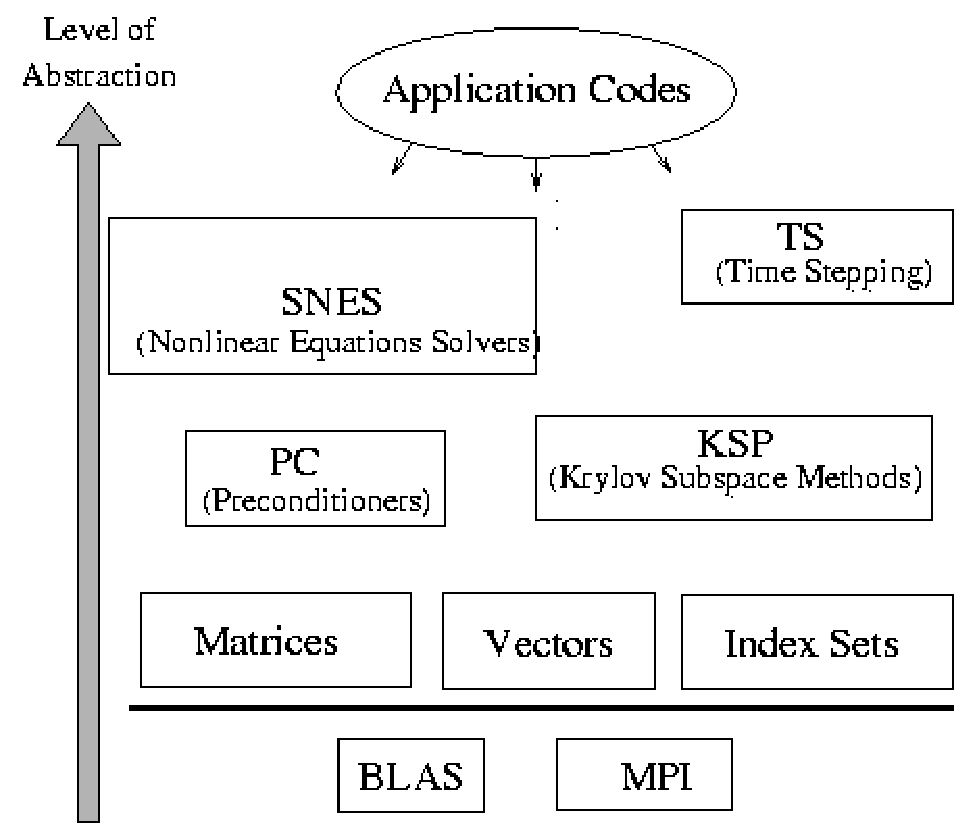
\includegraphics[width=8cm]{petscwww.eps}
\caption{\label{fig:petsc}Organization of the \petsc\ toolkit.}
\end{figure}

	\petsc\ components are discussed in detail in the users manual \citep{Balay:2002:PUM}. Each component manipulates a particular family of objects (for instance, vectors) and the operations one would like to perform on the objects. 
	The three basic abstract data objects are index sets, vectors and matrices. Built on top of this foundation are various classes of solver objects, which encapsulate virtually all information regarding the solution procedure for a particular class of problems, including the local state and various options such as convergence tolerances, etc. 
Some of the \petsc\ modules deal with 
\begin{itemize} 
\item index sets, including permutations, for indexing into vectors, renumbering, etc;
\item vectors;
\item matrices (generally sparse);
\item distributed arrays (useful for parallelizing regular grid-based problems);
\item Krylov subspace methods;
\item preconditioners, including multigrid and sparse direct solvers;
\item nonlinear solvers; and
\item timesteppers for solving time-dependent (nonlinear) PDEs.
\end{itemize}
Each of these components consists of an abstract interface (simply a set of calling sequences) and one or more implementations using particular data structures. \petsc\ is written in C, which lacks direct support for object-oriented programming. However, it is still possible to take advantage of the three basic principles of object-oriented programming to manage the complexity of such a large package. \petsc\ uses data encapsulation in both vector and matrix data objects. Application code access data through function calls. Also, all the operations are supported through polymorphism. The user calls a generic interface routine which then selects the underlying routine which handles the particular data structure. This is implemented by structures of function pointers. Finally, \petsc\ also uses inheritance in its design. All the objects are derived from an abstract base object. From this fundamental object, an abstract base object is defined for each \petsc\ object (\texttt{Mat}, \texttt{Vec} and so on) which in turn has a variety of instantiations that, for example, implement different matrix storage formats.

	\petsc\ provides clean and effective codes for the various phases of solving PDEs, with a uniform approach for each class of problems.  This design enables easy comparison and use of different algorithms (for example, to experiment with different Krylov subspace methods, preconditioners, or truncated Newton methods). Hence, \petsc\ provides a rich environment for modeling scientific applications as well as for rapid algorithm design and prototyping.

	Options can be specified by means of calls to subroutines in the source code and also as command-line arguments. Runtime options allow the user to test different tolerances, for example, without having to recompile the program. Also, since \petsc\ provides a uniform interface to all of its linear solvers ---the Conjugate Gradient, GMRES, etc. --- and a large family of preconditioners ---block Jacobi, overlapping additive Schwarz, etc. ---, one can compare several combinations of method and preconditioner by simply specifying them at execution time.
	
	The components enable easy customization and extension of both algorithms and implementations.  This approach promotes code reuse and flexibility, and separates the issues of parallelism from the choice of algorithms.  The \petsc\ infrastructure creates a foundation for building large-scale applications.
	Other advantages of \petsc\ are the following:
	\begin{itemize}
	\item High portability due to an elaborate Makefile system. Different architecture builds can coexist in the same installation. Where available, dynamic libraries are used to reduce disk space of executable files.
	\item Support for debugging and profiling: attachment to external debuggers, event logging, subroutine timing, convergence monitoring, etc. \petsc\ also has built-in graphics capabilities which allow for sparse pattern visualization, graphic convergence monitoring, operator's spectrum visualization and other user-defined operations.
	\item Programming interface for Fortran.
	\end{itemize}

%---------------------------------------------------
\chapter{Catalog of Solvers}
\label{cap:meth}

	This appendix provides a short description of all the eigensolvers which are available in \slepc, including the interfaces to external libraries. In the case of ``native'' methods, that is, those methods that are implemented directly in \slepc, the description includes a sketch of the algorithm which is actually implemented. A short description of wrappers to external libraries is provided in section \ref{sec:wrap} of this appendix, including pointers to the respective websites from which the software can be downloaded. In both cases, the description may also include method-specific parameters, that can be set in the same way as other \slepc options, either procedurally or via the command-line.

	Table \ref{tab:defaults} summarizes all eigensolvers available in \slepc, both native and external. This table shows the default values for some of the parameters that the user can adjust.
\begin{table}
\centering
\begin{tabular}{cccc} \hline
Method   & \texttt{ncv} & \texttt{max\_it} & \texttt{tol} \\ \hline
\texttt{lapack}   &  $nev$ &         -         &    -      \\ 
\texttt{power}    &  $nev$ & $\max(2000,100N)$ & $10^{-7}$ \\ 
\texttt{subspace} &  $\max(2\cdot nev,nev+15)$ & $\max(100,N)$ & $10^{-7}$ \\ 
\texttt{arnoldi}  &  $\max(2\cdot nev,nev+15)$ & $\max(100,N)$ & $10^{-7}$ \\ 
\hline
\texttt{arpack}   &  $\min(\max(20,2\!\cdot\!nev\!+\!\!1),N)$ & $\max(300,\lceil 2N/ncv\rceil)$ & $10^{-7}$ \\ 
\texttt{blzpack}  &  $\min(nev\!+\!\!10,2\!\cdot\!nev)$ & $\max(100,N)$ & $10^{-7}$ \\ 
\texttt{planso}   &  $nev$ & $\max(100,N)$ & $10^{-7}$ \\ 
\texttt{trlan}    &  $nev$ & $\max(100,N)$ & $10^{-7}$ \\ \hline
\end{tabular}
\caption{\label{tab:defaults}Default parameter values for all eigensolvers available in \slepc.}
\end{table}

	Table \ref{tab:support} summarizes the scope of each eigensolver by listing which portion of the spectrum can be selected (as defined in table \ref{tab:portion}), which problem types are supported (as defined in table \ref{tab:ptype}) and whether they are available or not in the complex version of \slepc. 
\begin{table}
\centering
\begin{tabular}{ccccc} \hline
Method   &  Portion of spectrum & Problem type & Complex \\ \hline
\texttt{lapack}   &  all                 & all & yes \\ 
\texttt{power}    &  Largest $|\lambda|$ & all & yes \\ 
\texttt{subspace} &  Largest $|\lambda|$ & all & yes \\ 
\texttt{arnoldi}  &  Largest $|\lambda|$ & all & yes \\ 
\hline
\texttt{arpack}   &  all &  all & yes \\ 
\texttt{blzpack}  &  Smallest $\mathrm{Re}(\lambda)$ & \Verb!EPS_HEP!, \Verb!EPS_GHEP!  & no \\ 
\texttt{planso}   &  Largest and smallest $\mathrm{Re}(\lambda)$ & \Verb!EPS_HEP! & no \\ 
\texttt{trlan}    &  Largest and smallest $\mathrm{Re}(\lambda)$ & \Verb!EPS_HEP! & no \\ \hline
\end{tabular}
\caption{\label{tab:support}Supported problem types for all eigesolvers available in \slepc.}
\end{table}


\section{\ident{power}}

This eigensolver covers several well-known single-vector iteration methods such as the Power Iteration, the Inverse Iteration and the Rayleigh Quotient Iteration.

When using the default spectral transformation (\ident{STSHIFT}), this solver provides an implementation of the Power Iteration. This is the simplest vector iteration method. It consists in premultiplying an initial vector by matrix $A$ repeatedly. Under certain conditions, the iteration converges to the dominant eigenvector (the one associated to the largest eigenvalue in magnitude). Then the approximate eigenvalue can be obtained by computing the Rayleigh quotient. Once an eigenvector has converged, deflation can be used to reveal the next ones. Note that this method will fail in the case that there is no unique dominant eigenvalue. Convergence can be very slow if separation of the dominant eigenvalue with the rest is small.

\begin{algorithm}[Basic Power Method\label{alg:pot}]~\rm
\begin{tabbing}
Input: Operator $O\!P$ and initial vector $v_0$\\
Output: Approximate dominant eigenpairs $(\theta,v)$ \\
xxxx\=xxx\=xxxxxxxxxxxxxxx\=\kill
\> Set $y=v_0$\\
\> For $k=1,2,\ldots$\\
\> \> Deflate previously converged eigenvectors \\
\> \> $v=y/\|y\|_B$ \\
\> \> $y=O\!Pv$ \\
\> \> $\theta=(y,v)_B$ \\
\> \> if $\|y-\theta v\|_2 < |\theta| \cdot \mathrm{tol}$, accept eigenpair \\
\> end
\end{tabbing}
\end{algorithm}
In the algorithm above, matrix $O\!P$ represents the operator, which can be any of the expressions in table \ref{tab:op}. Thus, the algorithm can be converted to the Inverse Iteration by simply specifying the \texttt{sinvert} transformation.

The Inverse Iteration works with a constant shift, that is, the operator is $(A-\sigma B)^{-1}B$ throughout the iteration. However, it is possible to change this behaviour by requesting the use of \emph{variable} shifts. There are two possibilities: Rayleigh shifts and Wilkinson shifts. This option can be changed with the command-line option \Verb!-eps_power_shift_type! or specified in the program source with the function \ident{EPSPowerSetShiftType}. 

The first alternative (\Verb!rayleigh!) results in the well-known Rayleigh Quotient Iteration (RQI), where the new shift $\rho_k$ is computed as the Rayleigh quotient of the current approximate eigenvector $v$
\begin{equation}
\rho_k=R(v)=\frac{v^H\!\!Av}{v^H\!Bv}
\end{equation}
The rate of convergence of this strategy is quadratic in general and cubic when the problem is Hermitian. Note that changing the shift may imply refactorization of matrix $(A-\rho_k B)$.

The second alternative (\Verb!wilkinson!) uses a more sophisticated formula for the shift \citep{Parlett:1998:SEP}.

%---------------------------------------------------
\section{\ident{subspace}}

The Subspace Iteration method is a generalization of the Power Method to $m$ initial vectors. Ortogonality of vectors is enforced in order to avoid linear dependence.

The implementation currently available in \slepc is based on \srrit \citep{Bai:1997:ASF}. It performs a Rayleigh-Ritz projection procedure in order to improve convergence. Deflation is handled by locking converged eigenvectors. For better performance, orthogonalization and projection are performed only when necessary.

\begin{algorithm}[Subspace Iteration\label{alg:sub}]~\rm
\begin{tabbing}
Input: Operator $O\!P$ \\
Output: $m$ dominant Schur vectors $V$ and corresponding eigenvalues\\
xxxx\=xxx\=xxx\=xxxxxxxxxxxx\=\kill
\> Generate a set of initial orthonormal vectors $V\in\C^{n\times m}$\\
\> For $k=1,2,\ldots$\\
\> \> Perform a Rayleigh-Ritz Projection step (algorithm \ref{alg:rrp})\\
\> \> Check convergence of eigenvalues \\
\> \> Orthogonalization loop \\
\> \> \> Repeatedly compute $V = O\!P\, V$ \\
\> \> \> Orthogonalize columns of $V$ \\
\> \> end \\
\> end
\end{tabbing}
\end{algorithm}

\begin{algorithm}[Rayleigh-Ritz Projection\label{alg:rrp}]~\rm
\begin{tabbing}
Input: Operator $O\!P$ and set of vectors $V$\\
Output: Schur vectors $V$ and quasi-triangular matrix $T$ \\
xxxx\=xxx\=xxxxxxxxxxxxxxx\=\kill
\> $T=V^H O\!P\, V$ \\
\> Reduce to Hessenberg form: $T=U_1^HTU_1$ \\
\> Reduce to quasi-triangular form: $T=U_2^HTU_2$ \\
\> $U=U_1U_2$ \\
\> $V=VU$ 
\end{tabbing}
\end{algorithm}

%---------------------------------------------------
\section{\ident{arnoldi}}

The version of the Arnoldi method implemented in \slepc uses locking and explicit restart. The orthogonalization technique can be chosen as described in section \ref{sec:orthog}.

The implemented method (see algorithm \ref{alg:arn}) builds an Arnoldi factorization of order \Verb!ncv! by means of algorithm \ref{alg:basicarn}. Converged eigenpairs are locked and the iteration is restarted with the rest of the columns being the active columns for the next Arnoldi factorization. Currently, no filtering is applied to the vector used for restarting.

\begin{algorithm}[Explicitly Restarted Arnoldi\label{alg:arn}]~\rm
\begin{tabbing}
Input: Operator $O\!P$, initial vector $v_1$, and dimension of the subspace $ncv$ \\
Output: A partial Schur decomposition $O\!P\,V=VH$ \\
xxxx\=xxx\=xxx\=xxx\=xxxxxxxxxxxx\=\kill
\> Normalize $v_1$\\
\> Restart loop\\
\> \> Compute an $ncv$-step Arnoldi factorization (algorithm \ref{alg:basicarn})\\
\> \> Reduce $H$ to (quasi-)triangular form, $H\leftarrow UHU^T$\\
\> \> Compute eigenvectors of $H$, $Hy_i=y_i\theta_i$ \\
\> \> Compute residual norm estimates, $\tau_i=\beta |e_m^Ty_i|$ \\
\> \> Lock converged eigenpairs\\
\> \> $V=VU$\\
\> end\\
\end{tabbing}
\end{algorithm}

\begin{algorithm}[Basic Arnoldi Factorization\label{alg:basicarn}]~\rm
\begin{tabbing}
Input: Operator $O\!P$, number of steps $m$, and $V_k$, $H_k$ with $k<m$  \\
Output: $(V_m,H_m,f,\beta)$ so that $O\!P\,V_m-V_mH_m=fe_m^T$, $\beta=\|f\|_B$ \\
xxxx\=xxx\=xxx\=xxx\=xxxxxxxxxxxx\=\kill
\> For $j=k+1,\ldots,m-1$\\
\> \> $w=O\!Pv_j$ \\
\> \> Orthogonalize $w$ with respect to $V_j$ (obtaining $h_{1:j,j}$) \\
\> \> $h_{j+1,j}=\|w\|_B$ \\
\> \> $v_{j+1}=w/h_{j+1,j}$ \\
\> end \\
\> $f=O\!Pv_m$ \\
\> Orthogonalize $f$ with respect to $V_m$ (obtaining $h_{1:m,m}$) \\
\> $\beta=\|f\|_B$ \\
\end{tabbing}
\end{algorithm}

%---------------------------------------------------
%\section{\ident{lanczos}}
%
%\begin{algorithm}[Lanczos]~\rm
%\begin{tabbing}
%Input: Symmetric matrix $A$ and number of steps $k$ \\
%Output: $(V_k,T_k)$ being $\alpha_i$ and $\beta_i$ the diagonal and subdiagonal elements of $T_k$ \\
%xxxx\=xxx\=xxxxxxxxxxxxxxx\=\kill
%\> Choose a 1-norm vector $v_1$\\
%\> Initialize $\beta_1=0$, $v_0=0$\\
%\> For $j=1,2,\ldots,k$\\
%\> \> $w_j=Av_j-\beta_j v_{j-1}$ \\
%\> \> $\alpha_j=(w_j,v_j)$ \\
%\> \> $w_j=w_j-\alpha_j v_j$ \\
%\> \> $\beta_{j+1}=\|w_j\|_2$ \\
%\> \> $v_{j+1}=w_j/\beta_{j+1}$ \\
%\> end
%\end{tabbing}
%\end{algorithm}

%---------------------------------------------------
\section{Wrappers to External Libraries}
\label{sec:wrap}

	\slepc interfaces to several external libraries for the solution of eigenvalue problems. This section includes a short description of each of these packages as well as some hints for using them with \slepc.

	To use these eigensolvers, one needs to do the following.
	\begin{enumerate}
	\item Install the external software.
	\item Enable the utilization of the external software from \slepc by editing the file \Verb!${SLEPC_DIR}/bmake/${PETSC_ARCH}/packages!. For example, to use \arpack, one would specify the following variables with the appropriate paths:
	\begin{Verbatim}[fontsize=\small]
ARPACK_INCLUDE    = 
ARPACK_LIB        = -L/home/slepc/soft/ARPACK -lparpack -larpack
SLEPC_HAVE_ARPACK = -DSLEPC_HAVE_ARPACK
	\end{Verbatim}
	\item Build the \slepc libraries.
	\item Use the runtime option \Verb!-eps_type <type>! to select the solver.
	\end{enumerate}

	An exception to the above is \lapack, which should be enabled during the \petsc{} installation.

\section*{\underline{\lapack}}
	\begin{description}
	\item[References.]\citep{Anderson:1992:LUG}.
	\item[Website.] \url{http://www.netlib.org/LAPACK}.
	\item[Version.] 2.0 or later.
	\item[Summary.] \lapack\ (Linear Algebra PACKage) is a software package for the solution of many different dense linear algebra problems, including eigenvalue problems.

	\slepc explicitly creates the operator matrix in dense form and then the appropriate \lapack{} driver routine is invoked. Therefore, this interface should be used only for testing and validation purposes and not in a production code. The operator matrix is created by applying the operator to the columns of the identity matrix.

	Currently, only \lapack{} drivers for standard eigenvalue problems are
used. Generalized problems are transformed to standard ones.
	
	\item[Installation.]
	The \slepc interface to \lapack{} can be used directly.
	\end{description}

\section*{\underline{\arpack}}
	\begin{description}
	\item[References.]\citep{Lehoucq:1998:AUG}, \citep{Maschhoff:1996:PEP}.
	\item[Website.] \url{http://www.caam.rice.edu/software/ARPACK}.
	\item[Version.] Release 2 (plus patches).
	\item[Summary.] \arpack\ (ARnoldi PACKage) is a software package for the computation of a few eigenvalues and corresponding eigenvectors of a general $n\times n$ matrix $A$. It is most appropriate for large sparse or structured matrices, where structured means that a matrix-vector product $w \leftarrow Av$ requires order $n$ rather than the usual order $n^2$ floating point operations. 
	
	\arpack\ is based upon an algorithmic variant of the Arnoldi process called the Implicitly Restarted Arnoldi Method (IRAM). When the matrix $A$ is symmetric it reduces to a variant of the Lanczos process called the Implicitly Restarted Lanczos Method (IRLM). These variants may be viewed as a synthesis of the Arnoldi/Lanczos process with the Implicitly Shifted QR technique that is suitable for large scale problems. 

	It can be used for standard and generalized eigenvalue problems, both in real and complex arithmetic. It is implemented in Fortran 77 and it is based on the reverse communication interface. A parallel version, \parpack, is available with support for both MPI and BLACS.
	\item[Installation.]
	In order to use \arpack\ with \slepc, both the sequential version and the parallel version (\parpack) have to be installed. First, unbundle \texttt{arpack96.tar.gz}, then \texttt{parpack96.tar.gz}. Make sure you delete any \texttt{mpif.h} files that could exist in the directory tree. Also it is recommended to unpack the patch files \texttt{patch.tar.gz} and \texttt{ppatch.tar.gz}. After that, modify the \texttt{ARmake.inc} file and then compile the software with \texttt{make all}.
	\end{description}

\section*{\underline{\blzpack}}
	\begin{description}
	\item[References.]\citep{Marques:1995:BDU}.
	\item[Website.] \url{http://www.nersc.gov/\~{}osni/\#Software}.
	\item[Version.] 04/00.
	\item[Summary.] \blzpack\ (Block LancZos PACKage) is a standard Fortran 77 implementation of the block Lanczos algorithm intended for the solution of the standard eigenvalue problem $Ax=\mu x$ or the generalized eigenvalue problem $Ax=\mu Bx$, where A and B are real, sparse symmetric matrices. The development of this eigensolver was motivated by the need to solve large, sparse, generalized problems from free vibration analysis in structural engineering. Several upgrades were performed afterwards aiming at the solution of eigenvalue problems from a wider range of applications.

	\blzpack\ uses a combination of partial and selective re-orthogonalization strategies. It can be run in either sequential or parallel mode, by means of MPI or PVM interfaces, and it uses the reverse communication strategy.
	\item[Installation.] For the compilation of the \texttt{libblzpack.a} library, first check the appropriate architecture file in the directory \texttt{sys/MACROS} and then type \texttt{creator -mpi}.
	\item[Specific options.] The \slepc interface to this package allows the user to specify the block size with the function \ident{EPSBlzpackSetBlockSize} or at run time with the option \Verb!-eps_blzpack_block_size <size>!. Also, the function \ident{EPSBlzpackSetNSteps} can be used to set the maximum number of steps per run (also with \Verb!-eps_blzpack_nsteps!).

	For the spectrum slicing feature, \slepc allows the programmer to provide the computational interval with the option \Verb!-eps_blzpack_interval!, or with the function \ident{EPSBlzpackSetInterval} in the program source.
	\end{description}

\section*{\underline{\planso}}
	\begin{description}
	\item[References.]\citep{Wu:1997:PLM}.
	\item[Website.] \url{http://www.nersc.gov/research/SIMON/planso.html}.
	\item[Version.] 1.0 (07/1997).
	\item[Summary.] This package implements the Lanczos algorithm with partial re-orthogonalization for symmetric generalized eigenvalue problems. It is based on the sequential package \lanso\ maintained by B. Parlett. \planso\ is implemented in Fortran 77 using MPI and the user must provide functions for matrix-vector products.

The current version uses the Omega-recurrence to simulate the loss of orthogonality among the Lanczos vectors and maintains semiorthogonality.  This is sufficient to guarantee that eigenvalues are computed accurately, but under extreme conditions the eigenvectors may not be as accurate as the eigenvalues.
	\item[Installation.] Change \texttt{Make.inc} in the top level directory to set appropriate compiler and flags to use. Then type \texttt{make lib plib}.
	\end{description}

\section*{\underline{\trlan}}
	\begin{description}
	\item[References.]\citep{Wu:2001:TLM}.
	\item[Website.] \url{http://www.nersc.gov/\~{}kewu/trlan.html}.
	\item[Version.] 1.0 (03/1999).
	\item[Summary.] This package provides a Fortran 90 implementation of the dynamic thick-restart Lanczos algorithm. This is a specialized version of Lanczos that targets only the case in which one wants both eigenvalues and eigenvectors of a large real symmetric eigenvalue problem that cannot use the shift-and-invert scheme. In this case the standard non-restarted Lanczos algorithm requires to store a large number of Lanczos vectors which can cause storage problems and make each iteration of the method very expensive.

	\trlan{} requires the user to provide a matrix-vector multiplication routine. The parallel version uses MPI as the message passing layer. 
	\item[Installation.] To install this package, it is necessary to have access to a Fortran 90 compiler. The compiler name and the options used are specified in the file called \texttt{Make.inc}. To generate the library, type \texttt{make libtrlan\_mpi.a} in the \texttt{TRLan} directory.
	\end{description}



%---------------------------------------------------
\cleardoublepage
\fancyhead{}\fancyhead[LO,RE]{\nouppercase{\scriptsize \sffamily Bibliography}}
\addcontentsline{toc}{chapter}{Bibliography}

\bibliographystyle{engnat}
\bibliography{slepc}

\cleardoublepage
\fancyhead{}\fancyhead[LO,RE]{\nouppercase{\scriptsize \sffamily Index}}
\addcontentsline{toc}{chapter}{Index}
%%
%% This is file `slepc.cls',
%% 
%% This file is based on book.cls.
%% 
%% Copyright 1993 1994 1995 1996 1997 1998 1999
%% The LaTeX3 Project and any individual authors listed elsewhere
%% in this file.
%% 
%% This file is part of the LaTeX2e system.
%% ----------------------------------------
%% 
%% It may be distributed under the terms of the LaTeX Project Public
%% License, as described in lppl.txt in the base LaTeX distribution.
%% Either version 1.0 or, at your option, any later version.
%% \CharacterTable
%%  {Upper-case    \A\B\C\D\E\F\G\H\I\J\K\L\M\N\O\P\Q\R\S\T\U\V\W\X\Y\Z
%%   Lower-case    \a\b\c\d\e\f\g\h\i\j\k\l\m\n\o\p\q\r\s\t\u\v\w\x\y\z
%%   Digits        \0\1\2\3\4\5\6\7\8\9
%%   Exclamation   \!     Double quote  \"     Hash (number) \#
%%   Dollar        \$     Percent       \%     Ampersand     \&
%%   Acute accent  \'     Left paren    \(     Right paren   \)
%%   Asterisk      \*     Plus          \+     Comma         \,
%%   Minus         \-     Point         \.     Solidus       \/
%%   Colon         \:     Semicolon     \;     Less than     \<
%%   Equals        \=     Greater than  \>     Question mark \?
%%   Commercial at \@     Left bracket  \[     Backslash     \\
%%   Right bracket \]     Circumflex    \^     Underscore    \_
%%   Grave accent  \`     Left brace    \{     Vertical bar  \|
%%   Right brace   \}     Tilde         \~}
\NeedsTeXFormat{LaTeX2e}[1995/12/01]
\ProvidesClass{slepc}
              [1999/01/07 v1.4a
 Standard LaTeX document class]
\newcommand\@ptsize{}
\newif\if@restonecol
\newif\if@titlepage
\@titlepagetrue
\newif\if@openright
\newif\if@mainmatter \@mainmattertrue
\if@compatibility\else
\DeclareOption{a4paper}
   {\setlength\paperheight {297mm}%
    \setlength\paperwidth  {210mm}}
\DeclareOption{a5paper}
   {\setlength\paperheight {210mm}%
    \setlength\paperwidth  {148mm}}
\DeclareOption{b5paper}
   {\setlength\paperheight {250mm}%
    \setlength\paperwidth  {176mm}}
\DeclareOption{letterpaper}
   {\setlength\paperheight {11in}%
    \setlength\paperwidth  {8.5in}}
\DeclareOption{legalpaper}
   {\setlength\paperheight {14in}%
    \setlength\paperwidth  {8.5in}}
\DeclareOption{executivepaper}
   {\setlength\paperheight {10.5in}%
    \setlength\paperwidth  {7.25in}}
\DeclareOption{landscape}
   {\setlength\@tempdima   {\paperheight}%
    \setlength\paperheight {\paperwidth}%
    \setlength\paperwidth  {\@tempdima}}
\fi
\if@compatibility
  \renewcommand\@ptsize{0}
\else
\DeclareOption{10pt}{\renewcommand\@ptsize{0}}
\fi
\DeclareOption{11pt}{\renewcommand\@ptsize{1}}
\DeclareOption{12pt}{\renewcommand\@ptsize{2}}
\if@compatibility\else
\DeclareOption{oneside}{\@twosidefalse \@mparswitchfalse}
\fi
\DeclareOption{twoside}{\@twosidetrue  \@mparswitchtrue}
\DeclareOption{draft}{\setlength\overfullrule{5pt}}
\if@compatibility\else
\DeclareOption{final}{\setlength\overfullrule{0pt}}
\fi
\DeclareOption{titlepage}{\@titlepagetrue}
\if@compatibility\else
\DeclareOption{notitlepage}{\@titlepagefalse}
\fi
\if@compatibility
\@openrighttrue
\else
\DeclareOption{openright}{\@openrighttrue}
\DeclareOption{openany}{\@openrightfalse}
\fi
\if@compatibility\else
\DeclareOption{onecolumn}{\@twocolumnfalse}
\fi
\DeclareOption{twocolumn}{\@twocolumntrue}
\DeclareOption{leqno}{\input{leqno.clo}}
\DeclareOption{fleqn}{\input{fleqn.clo}}
\DeclareOption{openbib}{%
  \AtEndOfPackage{%
   \renewcommand\@openbib@code{%
      \advance\leftmargin\bibindent
      \itemindent -\bibindent
      \listparindent \itemindent
      \parsep \z@
      }%
   \renewcommand\newblock{\par}}%
}
\ExecuteOptions{letterpaper,10pt,twoside,onecolumn,final,openright}
\ProcessOptions
\input{bk1\@ptsize.clo}
\setlength\lineskip{1\p@}
\setlength\normallineskip{1\p@}
\renewcommand\baselinestretch{}
\setlength\parskip{0\p@ \@plus \p@}
\@lowpenalty   51
\@medpenalty  151
\@highpenalty 301
\setcounter{topnumber}{2}
\renewcommand\topfraction{.7}
\setcounter{bottomnumber}{1}
\renewcommand\bottomfraction{.3}
\setcounter{totalnumber}{3}
\renewcommand\textfraction{.2}
\renewcommand\floatpagefraction{.5}
\setcounter{dbltopnumber}{2}
\renewcommand\dbltopfraction{.7}
\renewcommand\dblfloatpagefraction{.5}
\if@twoside
  \def\ps@headings{%
      \let\@oddfoot\@empty\let\@evenfoot\@empty
      \def\@evenhead{\thepage\hfil\slshape\leftmark}%
      \def\@oddhead{{\slshape\rightmark}\hfil\thepage}%
      \let\@mkboth\markboth
    \def\chaptermark##1{%
      \markboth {\MakeUppercase{%
        \ifnum \c@secnumdepth >\m@ne
          \if@mainmatter
            \@chapapp\ \thechapter. \ %
          \fi
        \fi
        ##1}}{}}%
    \def\sectionmark##1{%
      \markright {\MakeUppercase{%
        \ifnum \c@secnumdepth >\z@
          \thesection. \ %
        \fi
        ##1}}}}
\else
  \def\ps@headings{%
    \let\@oddfoot\@empty
    \def\@oddhead{{\slshape\rightmark}\hfil\thepage}%
    \let\@mkboth\markboth
    \def\chaptermark##1{%
      \markright {\MakeUppercase{%
        \ifnum \c@secnumdepth >\m@ne
          \if@mainmatter
            \@chapapp\ \thechapter. \ %
          \fi
        \fi
        ##1}}}}
\fi
\def\ps@myheadings{%
    \let\@oddfoot\@empty\let\@evenfoot\@empty
    \def\@evenhead{\thepage\hfil\slshape\leftmark}%
    \def\@oddhead{{\slshape\rightmark}\hfil\thepage}%
    \let\@mkboth\@gobbletwo
    \let\chaptermark\@gobble
    \let\sectionmark\@gobble
    }
  \if@titlepage
  \newcommand\maketitle{\begin{titlepage}%
  \let\footnotesize\small
  \let\footnoterule\relax
  \let \footnote \thanks
  \null\vfil
  \vskip 60\p@
  \begin{center}%
    {\LARGE \@title \par}%
    \vskip 3em%
    {\large
     \lineskip .75em%
      \begin{tabular}[t]{c}%
        \@author
      \end{tabular}\par}%
      \vskip 1.5em%
    {\large \@date \par}%       % Set date in \large size.
  \end{center}\par
  \@thanks
  \vfil\null
  \end{titlepage}%
  \setcounter{footnote}{0}%
  \global\let\thanks\relax
  \global\let\maketitle\relax
  \global\let\@thanks\@empty
  \global\let\@author\@empty
  \global\let\@date\@empty
  \global\let\@title\@empty
  \global\let\title\relax
  \global\let\author\relax
  \global\let\date\relax
  \global\let\and\relax
}
\else
\newcommand\maketitle{\par
  \begingroup
    \renewcommand\thefootnote{\@fnsymbol\c@footnote}%
    \def\@makefnmark{\rlap{\@textsuperscript{\normalfont\@thefnmark}}}%
    \long\def\@makefntext##1{\parindent 1em\noindent
            \hb@xt@1.8em{%
                \hss\@textsuperscript{\normalfont\@thefnmark}}##1}%
    \if@twocolumn
      \ifnum \col@number=\@ne
        \@maketitle
      \else
        \twocolumn[\@maketitle]%
      \fi
    \else
      \newpage
      \global\@topnum\z@   % Prevents figures from going at top of page.
      \@maketitle
    \fi
    \thispagestyle{plain}\@thanks
  \endgroup
  \setcounter{footnote}{0}%
  \global\let\thanks\relax
  \global\let\maketitle\relax
  \global\let\@maketitle\relax
  \global\let\@thanks\@empty
  \global\let\@author\@empty
  \global\let\@date\@empty
  \global\let\@title\@empty
  \global\let\title\relax
  \global\let\author\relax
  \global\let\date\relax
  \global\let\and\relax
}
\def\@maketitle{%
  \newpage
  \null
  \vskip 2em%
  \begin{center}%
  \let \footnote \thanks
    {\LARGE \@title \par}%
    \vskip 1.5em%
    {\large
      \lineskip .5em%
      \begin{tabular}[t]{c}%
        \@author
      \end{tabular}\par}%
    \vskip 1em%
    {\large \@date}%
  \end{center}%
  \par
  \vskip 1.5em}
\fi
\newcommand*\chaptermark[1]{}
\setcounter{secnumdepth}{2}
\newcounter {part}
\newcounter {chapter}
\newcounter {section}[chapter]
\newcounter {subsection}[section]
\newcounter {subsubsection}[subsection]
\newcounter {paragraph}[subsubsection]
\newcounter {subparagraph}[paragraph]
\renewcommand \thepart {\@Roman\c@part}
\renewcommand \thechapter {\@arabic\c@chapter}
\renewcommand \thesection {\thechapter.\@arabic\c@section}
\renewcommand\thesubsection   {\thesection.\@arabic\c@subsection}
\renewcommand\thesubsubsection{\thesubsection .\@arabic\c@subsubsection}
\renewcommand\theparagraph    {\thesubsubsection.\@arabic\c@paragraph}
\renewcommand\thesubparagraph {\theparagraph.\@arabic\c@subparagraph}
\newcommand\@chapapp{\chaptername}
\newcommand\frontmatter{%
    \cleardoublepage
  \@mainmatterfalse
  \pagenumbering{roman}}
\newcommand\mainmatter{%
    \cleardoublepage
  \@mainmattertrue
  \pagenumbering{arabic}}
\newcommand\backmatter{%
  \if@openright
    \cleardoublepage
  \else
    \clearpage
  \fi
  \@mainmatterfalse}
\newcommand\part{%
  \if@openright
    \cleardoublepage
  \else
    \clearpage
  \fi
  \thispagestyle{plain}%
  \if@twocolumn
    \onecolumn
    \@tempswatrue
  \else
    \@tempswafalse
  \fi
  \null\vfil
  \secdef\@part\@spart}

\def\@part[#1]#2{%
    \ifnum \c@secnumdepth >-2\relax
      \refstepcounter{part}%
      \addcontentsline{toc}{part}{\thepart\hspace{1em}#1}%
    \else
      \addcontentsline{toc}{part}{#1}%
    \fi
    \markboth{}{}%
    {\centering
     \interlinepenalty \@M
     \normalfont
     \ifnum \c@secnumdepth >-2\relax
       \huge\bfseries \partname~\thepart
       \par
       \vskip 20\p@
     \fi
     \Huge \bfseries #2\par}%
    \@endpart}
\def\@spart#1{%
    {\centering
     \interlinepenalty \@M
     \normalfont
     \Huge \bfseries #1\par}%
    \@endpart}
\def\@endpart{\vfil\newpage
              \if@twoside
                \null
                \thispagestyle{empty}%
                \newpage
              \fi
              \if@tempswa
                \twocolumn
              \fi}
\newcommand\chapter{\if@openright\cleardoublepage\else\clearpage\fi
                    \thispagestyle{plain}%
                    \global\@topnum\z@
                    \@afterindentfalse
                    \secdef\@chapter\@schapter}
\def\@chapter[#1]#2{\ifnum \c@secnumdepth >\m@ne
                       \if@mainmatter
                         \refstepcounter{chapter}%
%                         \typeout{\@chapapp\space\thechapter.}%
\typeout{--------------\space Capitulo\space\thechapter\space--------------}
                         \addcontentsline{toc}{chapter}%
                                   {\protect\numberline{\thechapter}#1}%
                       \else
                         \addcontentsline{toc}{chapter}{#1}%
                       \fi
                    \else
                      \addcontentsline{toc}{chapter}{#1}%
                    \fi
                    \chaptermark{#1}%
                    \addtocontents{lof}{\protect\addvspace{10\p@}}%
                    \addtocontents{lot}{\protect\addvspace{10\p@}}%
                    \if@twocolumn
                      \@topnewpage[\@makechapterhead{#2}]%
                    \else
                      \@makechapterhead{#2}%
                      \@afterheading
                    \fi}
\def\@makechapterhead#1{%
  \vspace*{50\p@}%
%  {\parindent \z@ \raggedright \normalfont
  {\parindent \z@ \raggedleft \normalfont
    \ifnum \c@secnumdepth >\m@ne
      \if@mainmatter
%        \huge\bfseries \@chapapp\space \thechapter
%        \par\nobreak
%        \vskip 20\p@
\setlength{\fboxsep}{2mm}\fbox{\large\sc\@chapapp}\hspace*{-1.5mm}
\setlength{\fboxsep}{4mm}\setlength{\fboxrule}{.5mm}\fbox{\Huge\bfseries\thechapter} \par \raggedright
        \vskip 40\p@
      \fi
    \fi
    \interlinepenalty\@M
%    \Huge \bfseries #1\par\nobreak
%    \vskip 40\p@
    \huge\bf\sffamily #1\par\nobreak
    \hfill\rule{10cm}{1pt}
    \vskip 30\p@
  }}
\def\@schapter#1{\if@twocolumn
                   \@topnewpage[\@makeschapterhead{#1}]%
                 \else
                   \@makeschapterhead{#1}%
                   \@afterheading
                 \fi}
\def\@makeschapterhead#1{%
  \vspace*{50\p@}%
  {\parindent \z@ \raggedright
    \normalfont
    \interlinepenalty\@M
    \Huge \bfseries  #1\par\nobreak
    \vskip 40\p@
  }}
\newcommand\section{\@startsection {section}{1}{\z@}%
                                   {-3.5ex \@plus -1ex \@minus -.2ex}%
                                   {2.3ex \@plus.2ex}%
                                   {\normalfont\Large\bfseries}}
\newcommand\subsection{\@startsection{subsection}{2}{\z@}%
                                     {-3.25ex\@plus -1ex \@minus -.2ex}%
                                     {1.5ex \@plus .2ex}%
                                     {\normalfont\large\bfseries}}
\newcommand\subsubsection{\@startsection{subsubsection}{3}{\z@}%
                                     {-3.25ex\@plus -1ex \@minus -.2ex}%
                                     {1.5ex \@plus .2ex}%
                                     {\normalfont\normalsize\bfseries}}
\newcommand\paragraph{\@startsection{paragraph}{4}{\z@}%
                                    {3.25ex \@plus1ex \@minus.2ex}%
                                    {-1em}%
                                    {\normalfont\normalsize\bfseries}}
\newcommand\subparagraph{\@startsection{subparagraph}{5}{\parindent}%
                                       {3.25ex \@plus1ex \@minus .2ex}%
                                       {-1em}%
                                      {\normalfont\normalsize\bfseries}}
\if@twocolumn
  \setlength\leftmargini  {2em}
\else
  \setlength\leftmargini  {2.5em}
\fi
\leftmargin  \leftmargini
\setlength\leftmarginii  {2.2em}
\setlength\leftmarginiii {1.87em}
\setlength\leftmarginiv  {1.7em}
\if@twocolumn
  \setlength\leftmarginv  {.5em}
  \setlength\leftmarginvi {.5em}
\else
  \setlength\leftmarginv  {1em}
  \setlength\leftmarginvi {1em}
\fi
\setlength  \labelsep  {.5em}
\setlength  \labelwidth{\leftmargini}
\addtolength\labelwidth{-\labelsep}
\@beginparpenalty -\@lowpenalty
\@endparpenalty   -\@lowpenalty
\@itempenalty     -\@lowpenalty
\renewcommand\theenumi{\@arabic\c@enumi}
\renewcommand\theenumii{\@alph\c@enumii}
\renewcommand\theenumiii{\@roman\c@enumiii}
\renewcommand\theenumiv{\@Alph\c@enumiv}
\newcommand\labelenumi{\theenumi.}
\newcommand\labelenumii{(\theenumii)}
\newcommand\labelenumiii{\theenumiii.}
\newcommand\labelenumiv{\theenumiv.}
\renewcommand\p@enumii{\theenumi}
\renewcommand\p@enumiii{\theenumi(\theenumii)}
\renewcommand\p@enumiv{\p@enumiii\theenumiii}
\newcommand\labelitemi{\textbullet}
\newcommand\labelitemii{\normalfont\bfseries \textendash}
\newcommand\labelitemiii{\textasteriskcentered}
\newcommand\labelitemiv{\textperiodcentered}
\newenvironment{description}
               {\list{}{\labelwidth\z@ \itemindent-\leftmargin
                        \let\makelabel\descriptionlabel}}
               {\endlist}
\newcommand*\descriptionlabel[1]{\hspace\labelsep
                                \normalfont\bfseries #1}
\newenvironment{verse}
               {\let\\\@centercr
                \list{}{\itemsep      \z@
                        \itemindent   -1.5em%
                        \listparindent\itemindent
                        \rightmargin  \leftmargin
                        \advance\leftmargin 1.5em}%
                \item\relax}
               {\endlist}
\newenvironment{quotation}
               {\list{}{\listparindent 1.5em%
                        \itemindent    \listparindent
                        \rightmargin   \leftmargin
                        \parsep        \z@ \@plus\p@}%
                \item\relax}
               {\endlist}
\newenvironment{quote}
               {\list{}{\rightmargin\leftmargin}%
                \item\relax}
               {\endlist}
\if@compatibility
\newenvironment{titlepage}
    {%
      \cleardoublepage
      \if@twocolumn
        \@restonecoltrue\onecolumn
      \else
        \@restonecolfalse\newpage
      \fi
      \thispagestyle{empty}%
      \setcounter{page}\z@
    }%
    {\if@restonecol\twocolumn \else \newpage \fi
    }
\else
\newenvironment{titlepage}
    {%
      \cleardoublepage
      \if@twocolumn
        \@restonecoltrue\onecolumn
      \else
        \@restonecolfalse\newpage
      \fi
      \thispagestyle{empty}%
      \setcounter{page}\@ne
    }%
    {\if@restonecol\twocolumn \else \newpage \fi
     \if@twoside\else
        \setcounter{page}\@ne
     \fi
    }
\fi
\newcommand\appendix{\par
  \setcounter{chapter}{0}%
  \setcounter{section}{0}%
  \gdef\@chapapp{\appendixname}%
  \gdef\thechapter{\@Alph\c@chapter}}
\setlength\arraycolsep{5\p@}
\setlength\tabcolsep{6\p@}
\setlength\arrayrulewidth{.4\p@}
\setlength\doublerulesep{2\p@}
\setlength\tabbingsep{\labelsep}
\skip\@mpfootins = \skip\footins
\setlength\fboxsep{3\p@}
\setlength\fboxrule{.4\p@}
\@addtoreset {equation}{chapter}
\renewcommand\theequation
  {\ifnum \c@chapter>\z@ \thechapter.\fi \@arabic\c@equation}
\newcounter{figure}[chapter]
\renewcommand \thefigure
     {\ifnum \c@chapter>\z@ \thechapter.\fi \@arabic\c@figure}
\def\fps@figure{tbp}
\def\ftype@figure{1}
\def\ext@figure{lof}
\def\fnum@figure{\figurename~\thefigure}
\newenvironment{figure}
               {\@float{figure}}
               {\end@float}
\newenvironment{figure*}
               {\@dblfloat{figure}}
               {\end@dblfloat}
\newcounter{table}[chapter]
\renewcommand \thetable
     {\ifnum \c@chapter>\z@ \thechapter.\fi \@arabic\c@table}
\def\fps@table{tbp}
\def\ftype@table{2}
\def\ext@table{lot}
\def\fnum@table{\tablename~\thetable}
\newenvironment{table}
               {\@float{table}}
               {\end@float}
\newenvironment{table*}
               {\@dblfloat{table}}
               {\end@dblfloat}
\newlength\abovecaptionskip
\newlength\belowcaptionskip
\setlength\abovecaptionskip{10\p@}
\setlength\belowcaptionskip{0\p@}
\long\def\@makecaption#1#2{%
  \vskip\abovecaptionskip
  \sbox\@tempboxa{#1: #2}%
  \ifdim \wd\@tempboxa >\hsize
    #1: #2\par
  \else
    \global \@minipagefalse
    \hb@xt@\hsize{\hfil\box\@tempboxa\hfil}%
  \fi
  \vskip\belowcaptionskip}
\DeclareOldFontCommand{\rm}{\normalfont\rmfamily}{\mathrm}
\DeclareOldFontCommand{\sf}{\normalfont\sffamily}{\mathsf}
\DeclareOldFontCommand{\tt}{\normalfont\ttfamily}{\mathtt}
\DeclareOldFontCommand{\bf}{\normalfont\bfseries}{\mathbf}
\DeclareOldFontCommand{\it}{\normalfont\itshape}{\mathit}
\DeclareOldFontCommand{\sl}{\normalfont\slshape}{\@nomath\sl}
\DeclareOldFontCommand{\sc}{\normalfont\scshape}{\@nomath\sc}
\DeclareRobustCommand*\cal{\@fontswitch\relax\mathcal}
\DeclareRobustCommand*\mit{\@fontswitch\relax\mathnormal}
\newcommand\@pnumwidth{1.55em}
\newcommand\@tocrmarg{2.55em}
\newcommand\@dotsep{4.5}
\setcounter{tocdepth}{2}
\newcommand\tableofcontents{%
    \if@twocolumn
      \@restonecoltrue\onecolumn
    \else
      \@restonecolfalse
    \fi
    \chapter*{\contentsname
        \@mkboth{%
           \MakeUppercase\contentsname}{\MakeUppercase\contentsname}}%
    \@starttoc{toc}%
    \if@restonecol\twocolumn\fi
    }
\newcommand*\l@part[2]{%
  \ifnum \c@tocdepth >-2\relax
    \addpenalty{-\@highpenalty}%
    \addvspace{2.25em \@plus\p@}%
    \begingroup
      \parindent \z@ \rightskip \@pnumwidth
      \parfillskip -\@pnumwidth
      {\leavevmode
       \large \bfseries #1\hfil \hb@xt@\@pnumwidth{\hss #2}}\par
       \nobreak
         \global\@nobreaktrue
         \everypar{\global\@nobreakfalse\everypar{}}%
    \endgroup
  \fi}
\newcommand*\l@chapter[2]{%
  \ifnum \c@tocdepth >\m@ne
    \addpenalty{-\@highpenalty}%
    \vskip 1.0em \@plus\p@
    \setlength\@tempdima{1.5em}%
    \begingroup
      \parindent \z@ \rightskip \@pnumwidth
      \parfillskip -\@pnumwidth
      \leavevmode \bfseries
      \advance\leftskip\@tempdima
      \hskip -\leftskip
      #1\nobreak\hfil \nobreak\hb@xt@\@pnumwidth{\hss #2}\par
      \penalty\@highpenalty
    \endgroup
  \fi}
\newcommand*\l@section{\@dottedtocline{1}{1.5em}{2.3em}}
\newcommand*\l@subsection{\@dottedtocline{2}{3.8em}{3.2em}}
\newcommand*\l@subsubsection{\@dottedtocline{3}{7.0em}{4.1em}}
\newcommand*\l@paragraph{\@dottedtocline{4}{10em}{5em}}
\newcommand*\l@subparagraph{\@dottedtocline{5}{12em}{6em}}
\newcommand\listoffigures{%
    \if@twocolumn
      \@restonecoltrue\onecolumn
    \else
      \@restonecolfalse
    \fi
    \chapter*{\listfigurename
      \@mkboth{\MakeUppercase\listfigurename}%
              {\MakeUppercase\listfigurename}}%
    \@starttoc{lof}%
    \if@restonecol\twocolumn\fi
    }
\newcommand*\l@figure{\@dottedtocline{1}{1.5em}{2.3em}}
\newcommand\listoftables{%
    \if@twocolumn
      \@restonecoltrue\onecolumn
    \else
      \@restonecolfalse
    \fi
    \chapter*{\listtablename
      \@mkboth{%
          \MakeUppercase\listtablename}{\MakeUppercase\listtablename}}%
    \@starttoc{lot}%
    \if@restonecol\twocolumn\fi
    }
\let\l@table\l@figure
\newdimen\bibindent
\setlength\bibindent{1.5em}
\newenvironment{thebibliography}[1]
     {\chapter*{\bibname
        \@mkboth{\MakeUppercase\bibname}{\MakeUppercase\bibname}}%
      \list{\@biblabel{\@arabic\c@enumiv}}%
           {\settowidth\labelwidth{\@biblabel{#1}}%
            \leftmargin\labelwidth
            \advance\leftmargin\labelsep
            \@openbib@code
            \usecounter{enumiv}%
            \let\p@enumiv\@empty
            \renewcommand\theenumiv{\@arabic\c@enumiv}}%
      \sloppy
      \clubpenalty4000
      \@clubpenalty \clubpenalty
      \widowpenalty4000%
      \sfcode`\.\@m}
     {\def\@noitemerr
       {\@latex@warning{Empty `thebibliography' environment}}%
      \endlist}
\newcommand\newblock{\hskip .11em\@plus.33em\@minus.07em}
\let\@openbib@code\@empty
\newenvironment{theindex}
               {\if@twocolumn
                  \@restonecolfalse
                \else
                  \@restonecoltrue
                \fi
                \columnseprule \z@
                \columnsep 35\p@
                \twocolumn[\@makeschapterhead{\indexname}]%
                \@mkboth{\MakeUppercase\indexname}%
                        {\MakeUppercase\indexname}%
                \thispagestyle{plain}\parindent\z@
                \parskip\z@ \@plus .3\p@\relax
                \let\item\@idxitem}
               {\if@restonecol\onecolumn\else\clearpage\fi}
\newcommand\@idxitem{\par\hangindent 40\p@}
\newcommand\subitem{\@idxitem \hspace*{20\p@}}
\newcommand\subsubitem{\@idxitem \hspace*{30\p@}}
\newcommand\indexspace{\par \vskip 10\p@ \@plus5\p@ \@minus3\p@\relax}
\renewcommand\footnoterule{%
  \kern-3\p@
  \hrule\@width.4\columnwidth
  \kern2.6\p@}
\@addtoreset{footnote}{chapter}
\newcommand\@makefntext[1]{%
    \parindent 1em%
    \noindent
    \hb@xt@1.8em{\hss\@makefnmark}#1}
\newcommand\contentsname{Contents}
\newcommand\listfigurename{List of Figures}
\newcommand\listtablename{List of Tables}
\newcommand\bibname{Bibliography}
\newcommand\indexname{Index}
\newcommand\figurename{Figure}
\newcommand\tablename{Table}
\newcommand\partname{Part}
\newcommand\chaptername{Chapter}
\newcommand\appendixname{Appendix}
\def\today{\ifcase\month\or
  January\or February\or March\or April\or May\or June\or
  July\or August\or September\or October\or November\or December\fi
  \space\number\day, \number\year}
\setlength\columnsep{10\p@}
\setlength\columnseprule{0\p@}
\pagestyle{headings}
\pagenumbering{arabic}
\if@twoside
\else
  \raggedbottom
\fi
\if@twocolumn
  \twocolumn
  \sloppy
  \flushbottom
\else
  \onecolumn
\fi
\endinput
%%
%% End of file `slepc.cls'.

\cleardoublepage

\end{document}

